\documentclass[times, utf8, diplomski, numeric]{fer}
\usepackage{booktabs}
\usepackage{indentfirst}
\usepackage{hyperref} 
\usepackage{tikz}
\usepackage{tikzscale}
\usepackage{dsfont}
\usepackage{commath}
\usepackage{listings}
\usepackage{makecell}
\usepackage{pdfpages}
\usepackage{subcaption}

\usetikzlibrary{positioning}
\usetikzlibrary{trees}

\tikzstyle{node}=[ultra thin,circle,draw,minimum size=15pt,inner sep=0pt]
\tikzstyle{text}=[above]
\tikzstyle{line}=[thin]
\tikzstyle{boldline}=[very thick]

\renewcommand{\lstlistingname}{Pseudok\^{o}d}% Listing -> Algoritam
\renewcommand{\lstlistlistingname}{Popis psudokod\^{o}va}% List of Listings -> Popis algoritama 

\definecolor{codegreen}{rgb}{0,0.6,0}
\definecolor{codegray}{rgb}{0.5,0.5,0.5}
\definecolor{codepurple}{rgb}{0.58,0,0.82}
\definecolor{backcolour}{rgb}{0.95,0.95,0.92}
\definecolor{keyword}{rgb}{0,0,0}

\lstdefinestyle{mystyle}{
    backgroundcolor=\color{backcolour},
    commentstyle=\color{codegreen},
    keywordstyle=\bfseries\color{keyword},
    numberstyle=\tiny\color{codegray},
    stringstyle=\color{codepurple},
    basicstyle=\footnotesize,
    breakatwhitespace=false,
    breaklines=true,
    captionpos=b,
    keepspaces=true,
    numbers=left,
    numbersep=5pt,
    showspaces=false,
    showstringspaces=false,
    showtabs=false,
    tabsize=4,
    inputencoding=utf8,
    morekeywords={vrati, ako, za\_svaki, prekini\_petlju, ponavljaj, puta}
}    

\lstset{style=mystyle,texcl=true}
% set font translations
%\lstset{inputencoding=utf8}
\lstset{extendedchars=true}
\lstset{
    literate=%
    {ć}{{\'c}}1
    {č}{{\v{c}}}1
    {đ}{{\dj{}}}1
    {š}{{\v{s}}}1
    {ž}{{\v{z}}}1
    {Ć}{{\'C}}1
    {Č}{{\v{C}}}1
    {Đ}{{\DJ{}}}1
    {Š}{{\v{S}}}1
    {Ž}{{\v{Z}}}1
}


\begin{document}

\thesisnumber{2022}

\title{Pronalaženje Booleovih funkcija maksimalne nelinearnosti evolucijskim računanjem}
\author{Kristijan Vulinović}

\maketitle

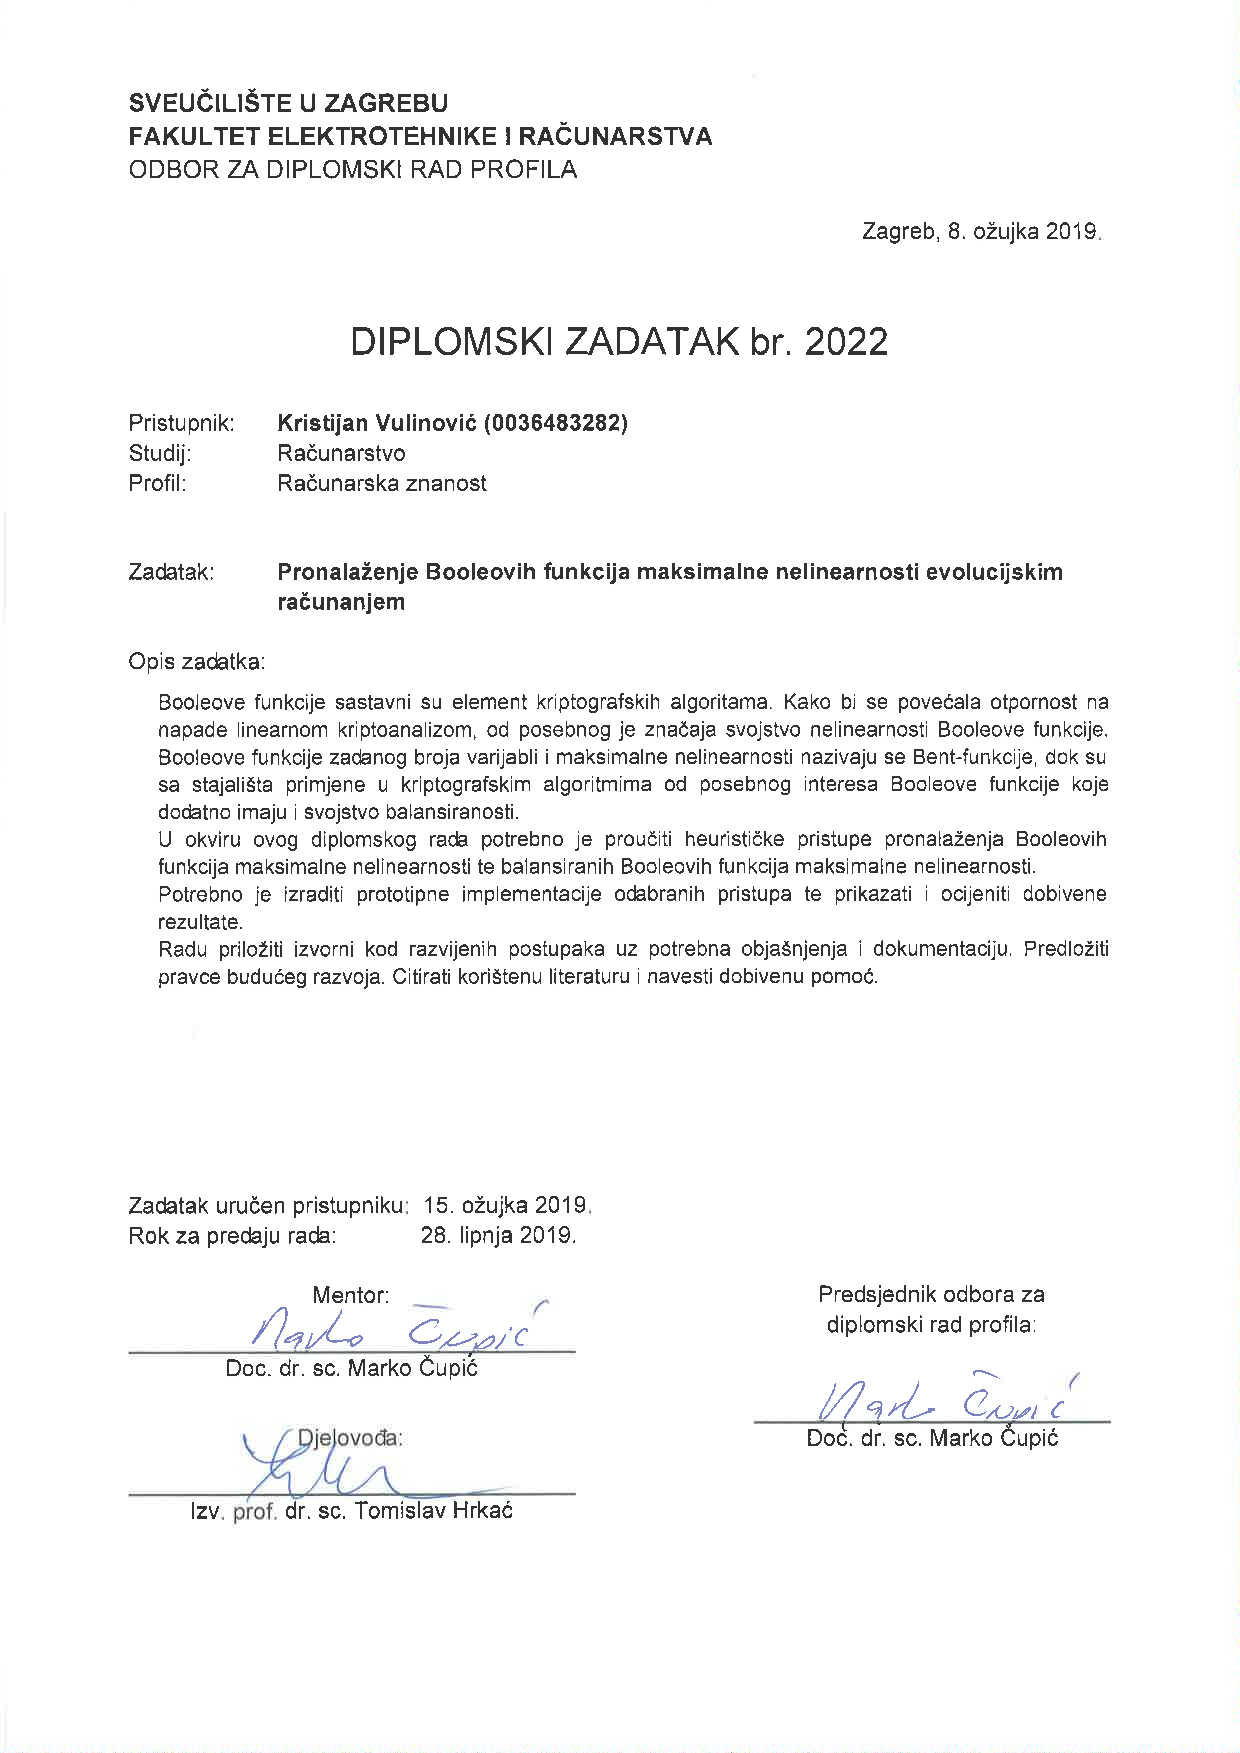
\includepdf{img/izvornik.pdf}

\zahvala{}

\tableofcontents

\chapter{Uvod}
Kriptografija je grana računarske znanosti, bez čijih dostignuća bi današnji svakodnevni život izgledao nezamislivo drugačije.
Većina se ljudi svakodnevno služi kriptografijom, makar toga nisu nužno ni svjesni.
Bilo to korištenjem online bankarstva, online trgovine ili jednostavno bilo kojeg online servisa temeljenog na \textit{HTTPS} protokolu.
Navedeni primjeri često se služe asimetričnim kriptografskim algoritmima kako bi klijent i poslužitelj razmijenili ključeve koje potom koriste u simetričnim kriptografskim algoritmima kojima se enkriptiraju njihove poruke.

Booleove funkcije predstavljaju jedan od sastavnih elemenata kriptografskih algoritama, poput na primjer S-kutija kod algoritma \textit{DES} i \textit{AES} \cite{daemen1999aes}.
Kako bi se postigla što veća sigurnost takvih sustava, potrebno je pomno odabrati korištene funkcije, ovisno o određenim svojstvima koje one posjeduju.
Jedan od najpoznatijih napada je napad linearnom kriptoanalizom, prvi puta opisan u \cite{golic1994linear}.
Kako bi se postigla veća otpornost na tu vrstu napada, od posebnog je značaja svojstvo nelinearnosti Booleove funkcije.
Pored toga, za primjenu u kriptografskim algoritmima dodatno je važno i svojstvo balansiranosti.
Osim navedenog, važna su i brojna druga svojstva poput svojstva korelacijske otpornosti \engl{correlation immunity}, autokorelacije \engl{autocorrelation}, algebarski stupanj \engl{algebraic degree}, algebarske otpornosti \engl{algebraic immunity} i drugih opisanih u \cite{CryptographicBooleanFunctions}.

Primarni fokus ovog rada je pronalazak Booleovih funkcija maksimalne nelinearnosti, kao i balansiranih Booleovih funkcija maksimalne nelinearnosti, pritom ne razmatrajući ostala svojstva.
Posebna pozornost posvećena je balansiranim Booleovim funkcijama sa $8$ varijabli, koje se koriste u algoritmu \textit{Achterbahn} \cite{gammel2005achterbahn}, kao i u algoritmu \textit{RAKAPOSHI} \cite{cid2009rakaposhi}, za koje je pitanje maksimalne moguće nelinearnosti još uvijek otvoreno.
Naime, najniža gornja granica nelinearnosti navedenih funkcija iznosi $118$, dok je najviša do sad pronađena nelinearnost u iznosu $116$.
\chapter{Booleove funkcije i interesantna svojstva}

Funkcija $f$ u općenitom je smislu definirana kao preslikavanje člana jednog skupa, koji se naziva domena u točno određeni član drugog skupa, koji se naziva kodomena.

Ako su domena i kodomena skup realnih brojeva $\mathds{R}$, funkcija $f : \mathds{R}^n \rightarrow \mathds{R}$ zove se \textbf{realna funkcija}.

\textbf{Booleova funkcija} je funkcija čija su domena i kodomena iz skupa $\mathds{B}$, što je skup elemenata $\mathds{B} = \{0, 1\}$.

\section{Načini prikaza}
Booleove funkcije moguće je jednoznačno definirati na brojne načine.
Najjednostavniji i često korišteni način je prikaz \textbf{tablicom istinitosti}, što je prikaz vrijednosti funkcije za sve moguće kombinacije varijabli, poredanih prema leksikografskom poretku vrijednosti ulaznih varijabli. 
\begin{table}
\centering
\begin{tabular}{ccc|c}
$x_1$ & $x_2$ & $x_3$ & $f(\vec{x})$ \\ \hline
 0 & 0 & 0 & 0 \\
 0 & 0 & 1 & 1 \\
 0 & 1 & 0 & 1 \\
 0 & 1 & 1 & 0 \\
 1 & 0 & 0 & 1 \\
 1 & 0 & 1 & 0 \\
 1 & 1 & 0 & 0 \\
 1 & 1 & 1 & 1
\end{tabular}
\caption{Primjer prikaza Booleove funkcije tablicom istinitosti}
\label{tbl:truth_table}
\end{table}
Tablica \ref{tbl:truth_table} predstavlja primjer prikaza Booleove funkcije $3$ varijable tablicom istinitosti.
Kako je redoslijed ulaznih varijabli u tablici istinitosti dogovoren, moguće je zapisivati samo zadnji stupac te istu funkciju prikazati kao \texttt{01101001}, što je zapis korišten u ostatku rada.

Osim tablice istinitosti postoje i kanonski oblici zapisivanja Booleovih funkcija, što se ostvaruje zapisivanjem varijabli i operacija koje nad njima djeluju.
Jedan od kanonskih oblika je suma minterma.
Minterm je izraz za kojega funkcija poprima vrijednost $1$ u samo jednom retku tablice istinitosti.
Unutar minterma, varijable su povezane operacijom AND, dok su mintermi međusobno povezani operacijom OR.
Zapis funkcije prikazane u tablici \ref{tbl:truth_table} kao suma minterma dan je u izrazu \eqref{eq:minterm}.
\begin{equation}\label{eq:minterm}
    f(x_1, x_2, x_3) = \bar{x}_1\bar{x}_2x_3 + \bar{x}_1x_2\bar{x}_3 + x_1\bar{x}_2\bar{x}_3 + x_1x_2x_3
\end{equation}

Izraz koji poprima vrijednost $0$ u samo jednom retku tablice istinitosti zove se maksterm.
Booleovu funkciju moguće je zapisati i kao umnožak maksterma, gdje su varijable unutar maksterma povezane operacijom OR, dok su makstermi međusobno povezani operacijom AND.
Zapis funkcije iz prethodnih primjera umnoškom maksterma prikazan je u izrazu \eqref{eq:maxterm}.
\begin{equation}\label{eq:maxterm}
    f(x_1, x_2, x_3) = \left(x_1 + x_2 + x_3\right) \cdot \left(x_1 + \bar{x}_2 + \bar{x}_3\right) \cdot \left(\bar{x}_1 + x_2 + \bar{x}_3\right) \cdot \left(\bar{x}_1 + \bar{x}_2 + x_3\right)
\end{equation}

Prikazani kanonski oblici koriste ukupno $3$ različite računske operacije; negaciju, AND i OR.
Booleovu funkciju je moguće zapisati i uz korištenje samo $2$ različite operacije, poput u zapisu u algebarskom normalnom obliku gdje se koriste samo operacije XOR i AND.
Zapis funkcije iz prethodnih primjera u algebarskom normalnom obliku prikazan je u izrazu \eqref{eq:anf}.
\begin{equation}\label{eq:anf}
    f(x_1, x_2, x_3) = x_1 \oplus x_2 \oplus x_3
\end{equation}

\begin{figure}[ht!] 
    \centering
    \includegraphics[width=.8\textwidth]{img/operator_tree}
    \captionsetup{justification=centering}
    \caption{Primjer prikaza Booleove funkcije stablom operatora}
    \label{fig:operator_tree}
\end{figure}
Svi opisani načini prikaza Booleovih funkcija posjeduju zajedničko svojstvo da svakoj funkciji odgovara točno jedan mogući prikaz.
To nije slučaj kod prikaza stablom operatora, gdje se funkcija grafički prikazuje kroz stablo, čiji s čvorovi operatori, a listovi varijable.
Svaki operator iz stabla primjenjuje se na djecu tog čvora.
Ovisno o korištenim operatorima, moguće je dobiti različite prikaze, a jedan od mogućih prikaza za prethodno korištenu funkciju dan je na slici \ref{fig:operator_tree}.
Stablo na slici izgrađeno je korištenjem operatora AND, OR, XOR i NOT.


\section{Svojstva Booleovih funkcija}

Realna funkcija $f$ je \textbf{linearna funkcija} ako je oblika:
\begin{equation}
    f(\vec{x}) = a_1x_1 + a_2x_2 + \dots + a_nx_n,
\end{equation}
gdje su $a_1, a_2, \dots, a_n \in \mathds{R}$, $x_1, x_2, \dots, x_n \in \mathds{R}$ te $f(\vec{x}) \in \mathds{R}$.

Realna funkcija je \textbf{afina funkcija} ako je oblika:
\begin{equation}\label{eq:affine_definition}
    f(\vec{x}) = a_0 + a_1x_1 + a_2x_2 + \dots + a_nx_n,
\end{equation}
gdje su $a_0, a_1, a_2, \dots, a_n \in \mathds{R}$, $x_1, x_2, \dots, x_n \in \mathds{R}$ te $f(\vec{x}) \in \mathds{R}$.

Slično kao i za realne funkcije, moguće je definirati linearnu i afinu Boolevou funkciju.
Pritom se umjesto operacija zbrajanja koristi operacija logičkog isključivo ili \engl{exclusive or}, odnosno XOR, dok se umjesto množenja koristi operacija konjunkcije, odnosno AND.

Booleova funkcija je linearna, ako je oblika:
\begin{equation}
    f(\vec{x}) = a_1x_1 \oplus a_2x_2 \oplus \dots \oplus a_nx_n,
\end{equation}
gdje su $a_1, a_2, \dots, a_n \in \mathds{B}$, $x_1, x_2, \dots, x_n \in \mathds{B}$ te $f(\vec{x}) \in \mathds{B}$.
Primjer linearne Booleove funkcije dan je u prethodno korištenoj funkciji \texttt{01101001}.
To svojstvo je teško primijetiti korištenjem prikaza tablice istinitosti, ali ga je trivijalno za primijetiti korištenjem algebarskog normalnog oblika, kao što se vidi iz izraza \eqref{eq:anf}.

Booleova funkcija je afina, ako je oblika:
\begin{equation}
    f(\vec{x}) = a_0 \oplus a_1x_1 \oplus a_2x_2 \oplus \dots \oplus a_nx_n,
\end{equation}
gdje su $a_0, a_1, a_2, \dots, a_n \in \mathds{B}$, $x_1, x_2, \dots, x_n \in \mathds{B}$ te $f(\vec{x}) \in \mathds{B}$.
Za svaku linearnu Booleovu funkciju vrijedi da je ona ujedno i afina Booleova funkcija, zbog čega je i prethodno spomenuta funkcija afina.
Obrat tvrdnje ne vrijedi, te je recimo funkcija \texttt{10010110} afina Booleova funkcija, ali nije linearna, što se vidi iz prikaza u algebarskom normalnom obliku danom u izrazu \eqref{eq:affine_function}.
\begin{equation} \label{eq:affine_function}
    f(\vec{x}) = 1 \oplus x_1 \oplus x_2 \oplus x_3,
\end{equation}

Booleova funkcija je \textbf{balansirana} ako u tablici istinitosti sadrži jednak broj vrijednosti $0$ i vrijednosti $1$.
Funkcija prikazana tablicom \ref{tbl:truth_table} je balansirana jer u svojoj tablici istinitosti sadrži $4$ nule i $4$ jedinice.
Funkcija \texttt{00100101} nije balansirana jer u tablici istinitosti ima $5$ nula, a samo $3$ jedinice. 

Za dvije Booleove funkcije, definirana je \textbf{Hammingova udaljenost} kao broj bitova po kojima se njihove tablice istinitosti međusobno razlikuju.
Tako je na primjer Hammingova udaljenost funkcija $f_1 =$ \texttt{01001011} i $f_2 =$ \texttt{00100111} iznosi $4$, jer se funkcije razlikuju u drugom, trećem, petom i šestom bitu.

\textbf{Nelinearnost} Booleove funkcije definirana je kao minimalna Hammingova udaljenost od svih afinih Booleovih funkcija.

Booleova funkcija $f$ je \textbf{Bent-funkcija} ako za dani broj varijabli posjeduje svojstvo maksimalne nelinearnosti te je jednako udaljena od svih afinih Booleovih funkcija.
Bent funkcija postoje samo za paran broj varijabli, ali postoji i skupina semi-bent-funkcija definirana za neparan broj varijabli, što je opisano u knjizi \cite{CryptographicBooleanFunctions}.

Na primjeru funkcije s dvije varijable, postoji ukupno $8$ afinih funkcija.
To su redom: \\*
\begin{minipage}[t]{.5\textwidth}
    \begin{equation*}
        \begin{aligned}
            f_1(\vec{x}) &= 0\\
            f_2(\vec{x}) &= x_1\\
            f_3(\vec{x}) &= x_2\\
            f_4(\vec{x}) &= x_1 \oplus x_2\\
        \end{aligned}
    \end{equation*}
\end{minipage}%
\begin{minipage}[t]{.5\textwidth}
    \begin{equation*}
        \begin{aligned}
            f_5(\vec{x}) &= 1\\
            f_6(\vec{x}) &= 1 \oplus x_1\\
            f_7(\vec{x}) &= 1 \oplus x_2\\
            f_8(\vec{x}) &= 1 \oplus x_1 \oplus x_2.\\
        \end{aligned}
    \end{equation*}
\end{minipage}
Radi jednostavnosti izračuna Hammingove udaljenosti, u nastavku je dan prikaz afinih Booleovih funkcija dviju varijabli korištenjem tablice istinitosti.\\*
\begin{minipage}[t]{.5\textwidth}
    \begin{equation*}
        \begin{aligned}
            f_1(\vec{x}) &= 0000\\
            f_2(\vec{x}) &= 0011\\
            f_3(\vec{x}) &= 0101\\
            f_4(\vec{x}) &= 0110\\
        \end{aligned}
    \end{equation*}
\end{minipage}%
\begin{minipage}[t]{.5\textwidth}
    \begin{equation*}
        \begin{aligned}
            f_5(\vec{x}) &= 1111\\
            f_6(\vec{x}) &= 1100\\
            f_7(\vec{x}) &= 1010\\
            f_8(\vec{x}) &= 1001\\
        \end{aligned}
    \end{equation*}
\end{minipage}
Na primjeru funkcije \texttt{1011}, moguće je izračunati da Hammingova udaljenost te funkcije od navedenih afinih funkcija iznosi redom: $3$, $1$, $3$, $3$, $1$, $3$, $1$ i $1$.
Najmanja udaljenost iznosi $1$, zbog čega i nelinearnost funkcije \texttt{1011} iznosi također $1$.
Kako je udaljenost od svake grupe afinih funkcija jednaka (pritom se istom grupom smatraju funkcije $f_1$ i $f_2$ za koje vrijedi da je $f_1 = 1 \oplus f_2$), ova funkcija je ujedno i Bent-funkcija.

\section {Walshov spektar}
Walshova transformacija Booleove funkcije $f$ definirana je kao:
\begin{equation}\label{eq:walsh transform}
    W_f(\vec{w}) = \sum_{\vec{x} \in \mathds{B}^n}f(\vec{x})(-1)^{\vec{w}\vec{x}},
\end{equation}
čime je definiran Walshov koeficijent $W_f(\vec{w})$.
Skup Walshovih koeficijenata za sve $\vec{w} \in \mathds{B}^n$, zove se \textbf{Walshov spektar} Booleove funkcije \cite{CryptographicBooleanFunctions}.

Svaki Walshov koeficijent predstavlja neočekivanu udaljenost \engl{unexpected distance} \cite{MeasuringBoolean} Booleove funkcije $f$ od pripadne linearne Booleove funkcije.
Za svaki par Booleovih funkcija, očekivana vrijednost Hammingove udaljenosti iznosi pola od ukupnog broja bitova u tablici istinitosti, odnosno $2^{n-1}$.
Neočekivana udaljenost definirana je kao razlika stvarne Hammingove udaljenosti dviju funkcija i njihove očekivane udaljenosti.

Na primjeru funkcije čija je tablica istinitosti $00111010$, Walshov koeficijent za $\vec{v} = 010$, odgovara neočekivanoj udaljenosti od linearne funkcije $f(\vec{x}) = x_1$, čija je tablica istinitosti jednaka $00110011$.
Kako je riječ o funkcijama $3$ varijable, očekivana udaljenost iznosi $2^{3-1} = 4$, dok je stvarna Hammingova udaljenost $2$.
Razlika te dvije vrijednosti daje $-2$, što je vrijednost neočekivane udaljenosti dane funkcije, kao i pripadni Walshov koeficijent.

Walshov spektar moguće je izračunati direktno korištenjem izraza \eqref{eq:walsh transform}, što je moguće izvesti u vremenskoj složenosti $\mathcal{O}(n^2)$.
Isto je moguće izračunati u vremenskoj složenosti $\mathcal{O}(n\log n)$ korištenjem brze Walshove transformacije \engl{fast Walsh transform}.
Taj se postupak provodi uzastopnom primjenom operatora koji za par brojeva $(a, b)$, računa novi par $(a', b')$ prema izrazu:
\begin{equation}\label{eq:fwt}
    (a', b') = (a+b, a-b).
\end{equation}
\begin{figure}[ht!] 
    \centering
    \includegraphics[width=.6\textwidth]{img/fwt_example}
    \captionsetup{justification=centering}
    \caption{Primjer izračuna brze Walshove transformacije nad Booleovom funkcijom čija je tablica istinitosti $00111010$}
    \label{fig:fwt_example}
\end{figure}
Na slici \ref{fig:fwt_example} prikazan je cjelokupni postupak izračuna brze Walshove transformacije za prethodno prikazanu funkciju.
Postupak se provodi u $\log n$ koraka, a svaki je korak prikazan jednim stupcem u slici.
Stupci na slici međusobno su povezani linijama koje prikazuju iz kojih brojeva je izračunat broj u pojedinom stupcu.
Točnije, svaki broj je povezan s točno $2$ broja iz prethodnog stupca, što ukazuje na to da je on dobiven zbrojem ili razlikom ta dva broja, u skladu s operatorom \eqref{eq:fwt}.
Prvi stupac prikazuje Booleovu funkciju nad kojom se računa brza Walshova transformacija.
U prvom koraku algoritma, tablica istinitosti se dijeli na grupe veličine $2$, te se na svaku skupinu primjenjuje operator \eqref{eq:fwt}, čime se dobije rezultat prikazan u drugom stupcu slike.
Sljedeći korak koristi grupe veličine $4$ te se operator \eqref{eq:fwt} primjenjuje redom na sve parove međusobno udaljene za $2$.
Općenito vrijedi da se u $n$-tom koraku brojevi grupiraju u grupe veličine $2^n$, a operator \eqref{eq:fwt} se primjenjuje na one brojeve unutar grupe koji se nalaze na međusobnoj udaljenosti $2^{n-1}$.
Postupak se ponavlja sve dok u zadnjem koraku ne preostane samo jedna grupa koja uključuje sve brojeve.

Iz opisanog postupka, kao i iz slike \ref{fig:fwt_example} moguće je primijetiti važno svojstvo, točnije kako svaki bit tablice istinitosti utječe na iznos pojedinog Walshovog koeficijenta. 
Navedeno svojstvo prikazano je podebljanom linijom na slici, čime su prikazani svi bitovi koji su uključeni u izračun trećeg Walshovog koeficijenta.
Također se primjećuje kako vrijedi i obrat, odnosno da svaki pojedini bit utječe na sve vrijednosti Walshovog spektra.

Primjećuje se kako opisani postupak rezultira ispravnim Walshovim koeficijentima za cijeli Walshov spektar Booleove funkcije, osim za prvi koeficijent.
Dobiven prvi koeficijent odgovara Hammingovoj težini Booleove funkcije, odnosno broju jedinica u njezinoj tablici istinitosti.
Ova činjenica predstavlja dodatno kompliciranje postupka izračuna vrijednosti željenih svojstava, s obzirom na to da je prvi broj potrebno obrađivati na drugi način od ostatka spektra.
U radu \cite{MeasuringBoolean} taj je problem riješen tako da se na vrijednosti tablice istinitosti primijeni sljedeća transformacija:
\begin{equation}
    x' = -1^x.
\end{equation}
Na taj se način skup ${0, 1}$ preslikava u skup ${1, -1}$.
Postupak izračuna brze Walshove transformacije uz korištenje navedene transformacije ulaznih bitova prikazan je na slici \ref{fig:transformed_fwt_example}.
\begin{figure}[ht!] 
    \centering
    \includegraphics[width=.6\textwidth]{img/transformed_fwt_example}
    \captionsetup{justification=centering}
    \caption{Primjer izračuna brze Walshove transformacije nad Booleovom funkcijom čija je tablica istinitosti $00111010$ uz primjenu transformacije bitova}
    \label{fig:transformed_fwt_example}
\end{figure}
Novo dobiveni rezultati razlikuju se od prethodnih po predznaku i magnitudi.
Usprkos tome, rezultati u prikladniji zbog prvog koeficijenta koji po svojstvima odgovara ostalima.

Pomoću Walshovog spektra računaju se ostala svojstva Booleove funkcije.
Funkcija je balansirana ako je njezin prvi Walshov koeficijent jednak nuli \cite{MaximalNonlinearity}:
\begin{equation}
    W_f(\vec{0}) = 0.
\end{equation} 

Nelinearnost $N_f$ Booleove funkcije $f$ određena je apsolutno najvećim Walshovim koeficijentom prema izrazu \cite{MaximalNonlinearity}:
\begin{equation}
    N_f = 2^{n-1} - \frac{1}{2}\max_{\vec{w} \in \mathds{B}^n} \abs{W_f(\vec{w})}.
\end{equation}
Na primjeru funkcije prikazane u slici \ref{fig:transformed_fwt_example}, apsolutno najveći koeficijent iznosi $4$, odnosno $-4$ iz čega slijedi da je nelinearnost funkcije jednaka $N_f = 2^{3-1} - \frac{1}{2}4$, odnosno $N_f = 2$.

Za svaku Booleovu funkciju $f$ sa $n$ varijabli vrijedi Parsevalova jednakost koja glasi:
\begin{equation}
    \sum_{\vec{w}\in \mathds{B}^n} \left( W_f(\vec{w}) \right)^2 = 2^{2n}.
\end{equation} 
Iz toga slijedi da nelinearnost $N_f$ Bent-funkcije sa $n$ varijabli iznosi:
\begin{equation}
    N_f = 2^{n-1} - 2^{\frac{n}{2}-1}.
\end{equation}
\chapter{Pregled područja}
S obzirom na već spomenutu važnost i primjenu Booleovih funkcija, postoji velik broj provedenih istraživanja o metodama njihova pronalaska.
Booleove funkcije željenih svojstava moguće je stvoriti na tri konceptualno različita načina kao što je podijeljeno u radovima \cite{picek2016new} i \cite{CryptographicBoolean}, a to su: nasumičnim generiranjem, algebarskim konstrukcijama ili heurističkom pretragom.

Nasumično generiranje predstavlja najjednostavniji i najbrži način stvaranja nove Booleove funkcije.
Veliki nedostatak istoga je suboptimalnost rezultata, s obzirom na to da nasumične funkcije u većini slučajeva ne posjeduju željena svojstva.

S druge strane algebarska konstrukcija pruža mogućnost stvaranja funkcija poželjnih svojstava, bazirano na poznavanju funkcija manjeg broja varijabli koje zadovoljavaju određenja svojstva.
Te se funkcije nadograđuju ili međusobno nadovezuju kako bi se dobila funkcija većeg broja varijabli, a također sa željenim svojstvima.
Negativne strane algebarskih konstrukcija javljaju se u tome što unatoč dobrim rezultatima za funkcije određenih svojstava, ovi postupci pružaju mogućnost pronalaska samo određenih funkcija, te postoji mogućnost postojanja drugih, jednako dobrih ili boljih funkcija koje nije moguće dobiti na ovaj način.
Dodatno loše svojstvo ovog postupka primjećuje se prilikom potrebe za stvaranjem većeg broja različitih funkcija, gdje se druge metode pokazuju prikladnijima.
Konstrukcijski algoritmi nisu u fokusu ovog rada te nisu dodatno obrađeni, no široki pregled istih dan je u knjizi \cite{CryptographicBooleanFunctions}.

Treću skupinu algoritama predstavljaju heurističke metode pretrage.
Ove metode pružaju mogućnost stvaranja velikog broja različitih funkcija pogodnih svojstava.
Najčešći predstavnici ove skupine algoritama su algoritmi evolucijskog računanja, te postoje brojna istraživanja o efikasnosti pojedine vrste algoritma, kao i načina zapisa funkcije i evaluacije iste.

U radu \cite{OnBentFunctions} po prvi puta se spominje pojam bent-funkcija, odnosno funkcija koje za zadani broj varijabli imaju maksimalnu moguću nelinearnost, te su jednako udaljene od svake afine funkcije.
U radu se također razmatra i Fourierova transformacija bent-funkcija, iz čega se dokazuje da bent-funkcije postoje samo za paran broj varijabli.

Mogućnost transformacije funkcije dodatno je istražena u \cite{MeasuringBoolean} gdje se opisuje postupak brze Walshove transformacije \engl{Fast Walsh Transform}.
Objašnjeno je i tumačenje dobivenih Walshovih koeficijenata u vidu udaljenosti od njima pripadnim afinim funkcijama, iz čega slijedi mogućnost izračuna nelinearnosti funkcije na temelju tako dobivenih koeficijenata.
Slično je prikazano i u radu \cite{CalculatingNonlinearity}, gdje se koristi Hadamardova matrica pomoću koje se računa Walshove transformacija.
Prikazan je rekurzivni postupak izračuna matrice te pseudok\^{o}d izračuna transformacije funkcije i njene nelinearnosti.

Rad \cite{millan1997smart} baziran je na metodi uspona na vrh \engl{hill climbing}.
Korištena metoda kreće od nasumično generirane funkcije te za nju računa Walshove koeficijente.
Kako bi se nelinearnost povećala, potrebno je smanjiti magnitudu koeficijenata najveće magnitude.
To je ostvareno tako da se za svaki bit iz tablice istinitosti računa koji se koeficijenti mijenjaju promjenom tog bita te se na kraju odabire jedan od bitova koji smanjuje ukupnu nelinearnost.
Ista metoda korištena je i u \cite{millan1997effective}, gdje je dodatno proširena tako da umjesto promjene samo jednog bita računa promjene Walshovih koeficijenata za promjenu svakog para bitova.
Na taj je način osigurano da se osim bent-funkcija mogu pronalaziti i balansirane Booleove funkcije visoke nelinearnosti.
Rad \cite{millan1998heuristic} prikazuje usporedbu do tada najboljih poznatih rezultata s rezultatima dobivenim kombinacijom genetskog algoritma i metode uspona na vrh.
Ista metoda dodatno je modificirana u radu \cite{millan1999boolean} gdje se uvode slabi \engl{weak requirements} i jaki \engl{strong requirements} zahtjevi, gdje slabi zahtjevi garantiraju kako se trenutno rješenje neće pogoršati u sljedećoj iteraciji algoritma, dok jaki zahtjevi pretpostavljaju poboljšanje rješenja.

Ponešto drugačiji pristup prikazan je u \cite{DiscoveryOfBent}.
Predstavljen je algoritam koji na temelju Walshovih koeficijenata za danu Booleovu funkciju dolazi do najbliže bent-funkcije, a da pritom ispituje promjene nad samo polovicom bitova iz tablice istinitosti funkcije.
Veliki nedostatak algoritma je mogućnost rada samo nad funkcijama koje imaju $4$ varijable, te nemogućnost skaliranja istoga na funkcije većeg broja varijabli.
\cite{DiscoveryOfBent} također ispituje mogućnosti iscrpne pretrage Booleovih funkcija korištenjem sklopa \textit{FPGA}.
Dobiveni rezultati ukazuju na visoko ubrzanje koje je moguće postići zahvaljujući paralelnom izračunu više funkcija korištenjem cjevovodne strukture \engl{pipeline}.
Unatoč dobivenom ubrzanju, pokazalo se kako nije moguće raditi iscrpnu pretragu za funkcije koje imaju više od $5$ varijabli.
Slični rezultati su dobiveni i u istraživanju \cite{EnumerationOfBentBoolean}, gdje autori također problemu pristupaju korištenjem sklopa \textit{FPGA}.
U radu se dodatno koristi i algebarski zapis Booleovih funkcija, za što je opisan postupak brze pretvorbe iz tablice istinitosti u algebarski zapis.

Autori u radu \cite{EvolvingBoolean} pomoću simuliranog kaljenja \engl{simulated annealing} \cite{SimulatedAnnealing} pretražuju funkcije koje zadovoljavaju više svojstava.
Traženjem balansirane Booleove funkcije s $8$ varijabli, dobiveno je rješenje nelinearnosti $116$, što je jednako trenutno najboljem poznatom rješenju.

Genetski algoritam \cite{holland1992adaptation} također je često korišten pristup, te su napisani brojni radovi o mogućim operatorima križanja i mutacije, kao i o primjeni na problem pronalaska Booleovih funkcija visoke nelinearnosti.
Rad \cite{manzoni2019balanced} uspoređuje $3$ različita operatora križanja primjenjiva na problem traženja balansiranih funkcija.
\cite{picek2014using} ispituje uspješnost genetskog algoritma korištenjem $3$ različita operatora mutacije, kao i $3$ različita operatora križanja.
U \cite{MaximalNonlinearity}, autori testiraju utjecaj različitih funkcija dobrote te ispituju težinu pronalaska balansirane Booleove funkcije maksimalne nelinearnosti s 8 varijabli.

Pored navedenih, korišteno je i genetsko programiranje \cite{koza1992genetic} u radovima \cite{picek2015cartesian}, \cite{picek2013evolving} i \cite{tesavr2010new}.
Autori u \cite{picek2015cartesian} dodatno koriste i kartezijsko genetsko programiranje te korištenjem skupa operatora OR, XOR, AND, XNOR i AND kojemu je jedan od ulaza negiran ostvaruju bolje rezultate nego li genetskim algoritmom na problemu generiranja S-kutija. 

\chapter{Pregled optimizacijskih algoritama}
\chapter{Analiza problema}
Pronalazak visoko nelinearnih Booleovih funkcija je poznat problem na kojemu je provedeno mnogo istraživanja.
Težina problema dolazi od veličine prostora stanja, koji raste super eksponencijalno s porastom broja varijabli.
Općenito vrijedi da za $n$ varijabli Booleova funkcija ima $2^n$ elemenata u tablici istinitosti te postoji $2^{2^n}$ različitih Booleovih funkcija.
Eksponencijalni rast tablice istinitosti također predstavlja implementacijske probleme zbog memorijskih zahtjeva za zapis istoga, ali i vremenskih zahtjeva za računanje.
Osim velikog prostora stanja, problem je i količina visoko nelinearnih Booleovih funkcija, odnosno to što je njihov udio u svim Booleovim funkcijama određenog broja varijabli sve manji s porastom broja varijabli.
Tako primjerice za $4$ varijabli postoji ukupno $65\:536$ Booleovih funkcija, od čega su $896$ funkcije Bent-funkcije, što čini $1.3\%$ svih funkcija.
Sa $6$ varijabli postoji ukupno $1.84 \times 10^{19}$ različitih Booleovih funkcija, od čega su $5\:425\:430\:528$ funkcije Bent-funkcije, što čini svega $2.94 \times 10^{-8}\%$ svih funkcije.
Za $8$ varijabli ovaj omjer postaje još manji te je samo $8.155 \times 10^{-44}\%$ \cite{DiscoveryOfBent}.
Za broj Bent-funkcija vrijedi ograda dana u izrazu \eqref{eq:bent_num} \cite{CryptographicBooleanFunctions}.
\begin{equation}\label{eq:bent_num}
    \left(2^{\frac{n}{2}}\right)! 2^{2^{\frac{n}{2}}} \leq
    \#bent \leq
    2^{2^{n-1}-\frac{1}{2}\binom{n}{\frac{n}{2}}}.
\end{equation}
Ukupan broj Booleovih funkcija, kao i ograde i stvaran broj Bent-funkcija za određene brojeve varijabli dan je u tablici \ref{tbl:boolean_count}.
\begin{table}[]
\begin{tabular}{c|cccc}
$n$ & donja ograda & broj Bent-funkcija & gornja ograda & broj Booleovih funkcija \\ \hline
$2$ & $8$ & $8$ & $8$ & $8$ \\
$4$ & $384$ & $896$ & $2\:048$ & $65\:536$ \\
$6$ & $2^{23.3}$ & $2^{32.3}$ & $2^{38}$ & $2^{64}$ \\
$8$ & $2^{95.6}$ & $2^{106.3}$ & $2^{129.2}$ & $2^{256}$ \\
$10$ & $2^{262.2}$ & $?$ & $2^{612}$ & $2^{1\:024}$
\end{tabular}
\caption{Ukupan broj Booleovih funkcija i ograde za Bent-funkcije (podatci preuzeti iz \cite{CryptographicBooleanFunctions})}
\label{tbl:boolean_count}
\end{table}

\section{Mjere vrednovanja rješenja}
Uz sve spomenute probleme prilikom pronalaska nelinearnih Booleovih funkcija, dodatan problem javlja se prilikom vrednovanja rješenja.
Korišteni optimizacijski algoritmi temelje se na tome da svakom rješenju dodjeljuju vrijednost u skladu s time koliko je ono dobro ili loše te pomoću te informacije pronalaze nova, potencijalno bolja rješenja.
Ovisno o vrsti mjere vrednovanja, one mogu biti ili mjere odnosno funkcije dobrote ili funkcije kazne.
Funkcije dobrote rješenju pridjeljuju vrijednost tako da ono rješenje koje je bolje dobije veću vrijednost, dok funkcije kazne veću vrijednost dodjeljuju onom rješenju koje je lošije.
Ovisno o tome koja vrsta funkcija vrednovanja se koristi, optimizacijski problem se postavlja kao maksimizacijski u slučaju funkcija dobrote, odnosno minimizacijski u slučaju funkcija kazne.

Najjednostavnija korištena mjera vrednovanja rješenja je upravo iznos nelinearnosti funkcije $N_f$.
Navedena mjera pruža jednostavno tumačenje uspješnosti rješenja.
Problem ovako definirane funkcije dobrote je u tome što velik broj različitih Booleovih funkcija posjeduje jednaku razinu nelinearnosti, zbog čega je postoje velika područja u kojima optimizacijski algoritmi nemaju informaciju o tome napreduju li ka boljem rješenju.

Sljedeća korištena mjera vrednovanja je nadogradnja prethodne tako da se osim nelinearnosti 
Booleove funkcije također vrednuje i iznos drugog po veličini Walshovog koeficijenta.
Ideja ove mjere je iskoristiti svojstvo Walshovih koeficijenata da predstavljaju udaljenosti od pojedinih afinih Booleovih funkcija.
Na taj se način od više funkcija jednake nelinearnosti prednost daje onima čija je udaljenost od sljedeće najbliže afine funkcije maksimalna.
Time je povećana vjerojatnost da povećavanje udaljenosti od trenutno najbliže afine funkcije rezultira i povećanjem nelinearnosti, jer neovisno o tome je li udaljenost od sljedeće najbliže afine funkcije povećana ili smanjena, ona je minimalna s obzirom na do tada pronađena rješenja.
Dodatna motivacija za ovako definiranom mjerom vrednovanja je u tome što je poznato da Bent-funkcije imaju sve Walshove koeficijente jednakog iznosa, što znači da je prilikom traženja Bent funkcija cilj minimizirati sve Walshove koeficijente, gledano po njihovoj apsolutnoj vrijednosti.

Treća korištena mjera vrednovanja dana je izrazom \eqref{eq:cost_function}, koja je korištena u mnogim radovima, poput: \cite{MaximalNonlinearity}, \cite{CryptographicBoolean}, \cite{EvolvingBoolean} i \cite{picek2016new}.
\begin{equation}\label{eq:cost_function}
    cost = \sum_{\vec{w}\in \mathds{B}^n} \abs{\abs{W_f(\vec{w)}} - X}^R
\end{equation}
Navedena mjera je funkcija kazne, koja se temelji na sličnom principu prethodne mjere vrednovanja, samo što se umjesto najveća dva koeficijenta Walshovog spektra koriste svi koeficijenti.
Funkcija posjeduje poželjna svojstva u vidu kažnjavanja velikih vrijednosti Walshovih koeficijenata, uz mogućnost utjecaja na način kažnjavanja kroz parametre $X$ i $R$.
Premda spomenuti parametri predstavljaju mogućnost podešavanja funkcije kazne, oni također predstavljaju i problem s obzirom na to da uvode potrebu za pomnim odabirom istih te ispitivanje njihovog utjecaja na rad optimizacijskih algoritama.
Za potrebe ovog rada korištene su vrijednosti $R=3$ te $X=4$, koje su se pokazale kao najuspješnije u dosadašnjim radovima \cite{EvolvingBoolean}.

\section{Analiza susjedstva}
Prije nego li se primijene optimizacijski algoritmi, potrebno je proučiti problem, ne bi li se pronašle određene pravilnosti ili karakteristike rješenja, a na temelju čega se može unaprijediti rad optimizacijskih algoritama.
S tim ciljem napravljena je vizualizacija susjedstva tako da je napravljena dvodimenzionalna matrica, gdje element $a_{i, j}$ bojom odgovara Hammingovoj udaljenosti Booleovih funkcija $f_i$ i $f_j$.
Opisani prikaz za slučaj funkcija s dvije varijable dan je na slici \ref{fig:function_2}. 
\begin{figure}[ht!] 
    \centering
    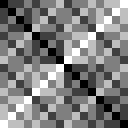
\includegraphics[width=.4\textwidth]{img/function_2}
    \captionsetup{justification=centering}
    \caption{Prikaz susjedstva za funkcije dviju varijabli}
    \label{fig:function_2}
\end{figure}
Konačna boja polja u matrici dobivena je skaliranjem Hammingovih udaljenosti na raspon od $0$ do $255$, te je tako dobiven broj korišten kao intenzitet sive boje.
Tako je primjerice na slici moguće primijetiti kako je glavna dijagonala crna, što je posljedica toga da ona prikazuje udaljenost funkcija od samih sebe, a ta udaljenost iznosi $0$, što rezultira crnom bojom.
Osim navedene glavne dijagonale, primjećuje se pravilnost i na sporednoj dijagonali, koja je naime u potpunosti bijela, što je posljedica toga da su to funkcije na najvećoj mogućoj udaljenosti.

\begin{figure}[!ht]
    \centering
    \begin{minipage}{.5\textwidth}
        \centering
        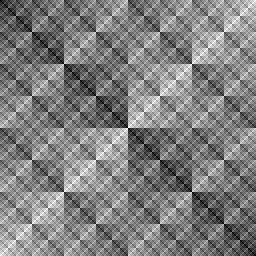
\includegraphics[width=.95\textwidth]{img/function_3}
        \captionsetup{justification=centering}
        \caption{Prikaz susjedstva za funkcije tri varijable}
        \label{fig:function_3}
    \end{minipage}%
    \begin{minipage}{.5\textwidth}
        \centering
        \includegraphics[width=.95\textwidth]{img/function_4}
        \captionsetup{justification=centering}
        \caption{Prikaz susjedstva za funkcije četiri varijable}
        \label{fig:function_4}
    \end{minipage}
\end{figure}

Na slici \ref{fig:function_3} grafički su prikazane udaljenosti funkcija tri varijable, dok slika \ref{fig:function_4} prikazuje udaljenosti za funkcije četiri varijable. 
Kako postoji ukupno $65\:536$ različitih Booleovih funkcija četiri varijable, nije moguće prikazati udaljenosti na prethodno opisano način jer bi tako dobivena slika zauzimala $4$GB prostora.
Kako bi dimenzije slike bile manje, umjesto da jedan slikovni element predstavlja udaljenost dviju funkcija, napravljeno je da jedan slikovni element predstavlja udaljenosti $8$ funkcija međusobno.
To je ostvareno tako da svaki element zapravo prikazuje aritmetičku sredinu onoga što bi prikazivalo područje od $8\times8$ elemenata u slici pune razlučivosti.

Na prikazanim slikama moguće je primijetiti određene pravilnosti.
Kao što je već spomenuto za sliku \ref{fig:function_2}, i na primjerima funkcija s većim brojem varijabli vrijedi to da je glavna dijagonala crna, dok je sporedna dijagonala bijela.
Osim toga, primjećuje se kako je sliku moguće podijeliti u kvadrate, tako je na primjer svaku sliku moguće podijeliti na $4$ kvadrata, svaki od tih kvadrata također je moguće podijeliti na $4$ daljnja kvadrata, i tako dalje.
Premda navedeno može djelovati kao potencijalno korisno svojstvo, isto je posljedica redoslijeda kojim su zapisane Booleove funkcije.
Na primjeru slike \ref{fig:function_3}, postoji ukupno $256$ različitih Booleovih funkcija.
Prvih $128$ funkcija ima $0$ kao prvi bit tablice istinitosti, dok drugih $128$ ima $1$ na mjestu prvog bita.
Ta promjena bita je razlog zbog kojeg je sliku moguće podijeliti na kvadrate upravo na mjestu gdje se mijenja vrijednost tog bita.
Manje kvadrate unutar slike moguće je objasniti na isti način, naime bit na drugom mjestu u tablici istinitosti imat će vrijednost $0$ za prve $64$ funkcije, nakon čega će imati vrijednost $1$ za sljedeće $64$ funkcija, nakon čega će opet imati vrijednost $0$ i tako dalje.
Ista pravilnost vrijedi za sve bitove tablice istinitosti, jedino što se frekvencija promjene vrijednosti bita povećava s većim indeksima bita u tablici istinitosti.

\begin{figure}[ht!] 
    \centering
    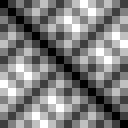
\includegraphics[width=.4\textwidth]{img/function_gray_2}
    \captionsetup{justification=centering}
    \caption{Prikaz susjedstva za funkcije dviju varijabli, za funkcije generirane korištenjem Grayevog k\^oda}
    \label{fig:function_gray_2}
\end{figure}
Kako su sve uočene pravilnosti u prethodnim slikama posljedica načina na koji su generirane Booleove funkcije, isproban je grafički prikaz u kojemu funkcije nisu zapisane leksikografskim redom u odnosu na njihove tablice istinitosti, već korištenjem Grayevog k\^oda.
Grayev k\^od je redoslijed zapisa Booleovih funkcija u kojemu se dvije susjedne funkcije uvijek razlikuju za točno jedan bit. 
Motivacija za prikazivanjem funkcija u ovom redoslijedu dolazi iz toga što su susjedne funkcije međusobno slične, zbog čega ne bi trebalo dolaziti do jednakih uzoraka udaljenosti kao u prethodnom zapisu.
Primjer na funkciji dvije varijable prikazan je na slici \ref{fig:function_gray_2}.

\begin{figure}[!ht]
    \centering
    \begin{minipage}{.5\textwidth}
        \centering
        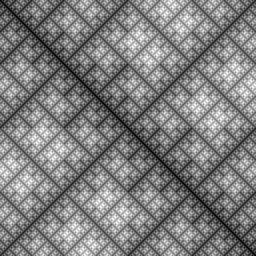
\includegraphics[width=.95\textwidth]{img/function_gray_3}
        \captionsetup{justification=centering}
        \caption{Prikaz susjedstva za funkcije tri varijable, za funkcije generirane korištenjem Grayevog k\^oda}
        \label{fig:function_gray_3}
    \end{minipage}%
    \begin{minipage}{.5\textwidth}
        \centering
        \includegraphics[width=.95\textwidth]{img/function_gray_4}
        \captionsetup{justification=centering}
        \caption{Prikaz susjedstva za funkcije četiri varijable, za funkcije generirane korištenjem Grayevog k\^oda}
        \label{fig:function_gray_4}
    \end{minipage}
\end{figure}


Slika \ref{fig:function_gray_3} prikazuje udaljenosti funkcija tri varijable, dok slika \ref{fig:function_gray_4} prikazuje udaljenosti funkcija četiri varijable.
Primjećuje se kako i u ovom redoslijedu zapisa funkcija postoje određene pravilnosti, točnije tamnija boja na dijagonalama.
Kao i kod leksikografskog poretka, glavna dijagonala je najtamnija jer prikazuje udaljenost funkcije od sebe same te je vrijednost tog polja $0$.
Sporedna dijagonala je također izrazito tamna, što je ponovno uzrokovano redoslijedom generiranja funkcija.
Naime, sporedna dijagonala prikazuje udaljenost dviju funkcija na međusobnoj udaljenosti $1$.
Sličan uzorak se ponavlja i na dijagonalama manjih kvadrata, dobivenih podjelom slike na četiri dijela.
Kako ni u ovom slučaju grafički prikaz nije omogućio pronalazak pravilnosti u svojstvima funkcija, osim redoslijeda kojim su generirane, ovi pristupi nisu korišteni u nastavku rada.

Osim grafičkih prikaza susjedstva, korisno je pogledati i funkcije grupirane tako da je za Booleovu funkciju prikazan popis svih Bent-funkcija koje su joj najbliže.
Motivacija tog prikaza je pronaći zajedničke dijelove najbližih Bent-funkcija te ustvrditi je li moguće odrediti koje bitove tablice istinitosti treba ili ne treba mijenjati kako bi se dobila funkcija veće nelinearnosti.
Prikaz Booleovih funkcija i njima najbližih Bent-funkcija za funkcije dvije varijable dan je u tablici \ref{tbl:neighbor}
\begin{table}[]
\centering
\begin{tabular}{ccccccccccc}
$0000$ & $0001$ &  & $0011$ & $0001$ &  & $0110$ & $1110$ &  & $0101$ & $0001$ \\
       & $0010$ &  &        & $0010$ &  &        & $0010$ &  &        & $1101$ \\
       & $0100$ &  &        & $1011$ &  &        & $0100$ &  &        & $0100$ \\
       & $1000$ &  &        & $0111$ &  &        & $0111$ &  &        & $0111$ \\
       &        &  &        &        &  &        &        &  &        &        \\
$1111$ & $1110$ &  & $1100$ & $1110$ &  & $1001$ & $0001$ &  & $1010$ & $1110$ \\
       & $1101$ &  &        & $1101$ &  &        & $1101$ &  &        & $0010$ \\
       & $1011$ &  &        & $0100$ &  &        & $1011$ &  &        & $1011$ \\
       & $0111$ &  &        & $1000$ &  &        & $1000$ &  &        & $1000$ \\
\end{tabular}
\caption{Popis Booleovih funkcija dvije varijable i njima najbližih Bent-funkcija}
\label{tbl:neighbor}
\end{table}
U danoj tablici primjećuje se pravilnost.
Točnije, svaka od prikazanih funkcija ima točno četiri Bent-funkcije koje su joj najbliže.
Usporede li se funkcije međusobno, primjećuje se da svaka funkcija ima par, odnosno drugu funkciju takvu da prva funkcija ima četiri njoj najbliže Bent-funkcije, dok druga funkcija ima druge četiri Bent-funkcije koje su joj najbliže.
Navedeni parovi funkcija su prikazani jedan ispod drugoga u tablici \ref{tbl:neighbor} te se primjećuje kako je jedna funkcija zapravo negacija druge funkcije.
Isto se primjećuje i za Bent-funkcije koje su najbliže navedenim funkcijama, gdje vrijedi da je Bent-funkcije najbliže prvoj funkciji moguće dobiti negiranjem Bent-funkcija najbližih drugoj funkciji.
Opisano svojstvo proizlazi iz definicije afinih Booleovih funkcija, dane u izrazu \eqref{eq:affine_definition}.
Ovisno o koeficijentu $a_0$, postoje dvije različite afine funkcije, jedna u kojoj je koeficijent $a_0$ jednak nuli, druga u kojoj je jednak jedinici.
Kako je koeficijent $a_0$ povezan operatorom XOR, on zapravo uzrokuje da za svaku afinu funkciju $f$, postoji afina funkcija $f-$ koja je jednaka negiranoj funkciji $f$.
Upravo iz tog razloga slijedi svojstvo da za svaku grupu funkcije i njoj pripadnih Bent-funkcija, postoji pripadna grupa dobivena negiranjem funkcija prethodne grupe.
Koristeći ovu činjenicu moguće je prostor pretrage smanjiti za pola, s obzirom na to da je dovoljno provjeriti jednu funkciju te ona ujedno daje informacije i za njoj komplementarnu funkciju.

Booleove funkcije dvije varijable korisne su za potrebe demonstracije jer ih je moguće sve prikazati, no ne pružaju vjeran uvid u problem, s obzirom na to da je točno pola funkcija afino, dok su preostale funkcije Bent-funkcije, s udaljenošću $1$ od najbliže afine funkcije.
Isti način grupiranja zato je primijenjen na Booleove funkcije četiri varijable.
Primjećuje se kako u ovom slučaju funkcije imaju različit broj Bent-funkcija koje su im najbliže, no postoje određene pravilnosti.

Najviše susjednih Bent-funkcija imaju upravo afine funkcije te vrijedi da svaka afina funkcija ima točno $448$ susjednih Bent-funkcija, što je pola od ukupnog broja Bent-funkcija četiri varijable.
Kod afinih funkcija vrijedi da promjena bilo kojeg bita tablice istinitosti povećava nelinearnost za jedan, zbog čega ove funkcije nisu korisne za daljnje razmatranje.
Za funkcije čija je nelinearnost jednaka jedan, moguće je primijetiti kako imaju uvijek jednak broj Bent-funkcija koje su im najbliže, točnije $168$.
Zanimljivo je primijetiti kako je ovdje moguće uočiti pravilnosti, tako primjerice za funkciju \texttt{0101010101010100} vrijedi da promjena bilo kojeg bita vodi prema funkciji veće nelinearnosti, osim promjene zadnjeg bita, što dovodi do afine funkcije čija je nelinearnost jednaka nuli.
Primjećuje se kako sve ostale funkcije također dolaze u pravilnim grupama, tako postoje funkcije koje imaju ukupno $64$ najbliže Bent-funkcije, funkcije koje imaju $56$, $16$, $4$ i $1$ najbližu Bent-funkciju.
Za svaku grupu definiranu na opisan način vrijedi da postoji skupina bitova zajednička svim Bent-funkcijama, što upućuje na postojanje skupina bitova unutar svake funkcije koju se ne smije mijenjati kako bi se postigla maksimalna moguća nelinearnost.
Zanimljivo je uočiti postojanje funkcija koje su svojevrsni lokalni optimum.
Na primjer, funkcija \texttt{0101000000001010} ima nelinearnost $4$, a promjenom bilo kojeg bita navedene funkcije dobiva se funkcija čija nelinearnost iznosi $3$.
Unatoč tome, navedena funkcija nije Bent-funkcija, odnosno postoje funkcije čija je nelinearnost veća.

Od iznimnog je interesa razviti postupak pronalaska bitova koje treba te bitova koje ne treba mijenjati, kako bi se ubrzali postupci pretrage.
U radovima \cite{millan1997smart} i \cite{millan1999boolean} opisan je postupak temeljen na brzoj Walshovoj transformaciji.
Opisani postupak zasniva se na tome da je jednom kad se izračunaju Walshovi koeficijenti za određenu Booleovu funkciju poznato koje koeficijente treba promijeniti i na koji način kako bi se ostvarila Booleova funkcija veće nelinearnosti.
Jedno moguće rješenje je da se za svaku funkciju nastalu promjenom samo jednog bita tablice istinitosti ponovno računa cijeli postupak brze Walshove transformacije, što je moguće napraviti u vremenskoj složenosti $\mathcal{O}(n\log n)$, gdje je $n$ broj bitova u tablici istinitosti.
Kako je to potrebno napraviti za svaku moguću promjenu, odnosno za svaki bit tablice istinitosti, ukupna složenost iznosi $\mathcal{O}(n^2\log n)$.
Umjesto toga, autori predlažu postupak u kojemu nakon promjene jednog bita tablice istinitosti nije potrebno provoditi cijelu Walshovu transformaciju, već samo ažurirati one brojeve koji se mijenjaju promjenom tog bita, što je moguće izvesti u vremenskoj složenosti $\mathcal{O}(n)$, čime je provjeru svih bitova moguće ostvariti u složenosti $\mathcal{O}(n^2)$.

Inspirirano opisanim postupkom, razmotreni su Walshovi koeficijenti Booleove funkcije, te način kako pomoću njih ustanoviti koje bitove je potrebno promijeniti.
Na primjeru funkcije \texttt{00000111}, Walshovi koeficijenti iznose $-2$, $-2$, $-2$, $-2$, $-6$, $2$, $2$, $2$, što je prikazano na slici \ref{fig:3_var_function}.
\begin{figure}[ht!] 
    \centering
    \includegraphics[width=.45\textwidth]{img/3_var_function}
    \captionsetup{justification=centering}
    \caption{Prikaz izračuna Walshovih koeficijenata za funkciju tri varijable}
    \label{fig:3_var_function}
\end{figure}
Slika ujedno prikazuje i međurezultate prilikom računanja koeficijenata, te su brojevi koji ovise jedan o drugome na slici povezani linijom.
Walshovi koeficijenti računati su u tri koraka, gdje je svaki korak redom prikazan od lijeva prema desno.
Istu transformaciju moguće je provesti i reverzno, od desna prema lijevo, čime se određuje koji bit tablice istinitosti kako utječe na pojedini Walshow koeficijent.
Kako bi se povećala nelinearnost funkcije, potrebno je smanjiti magnitudu najvećeg Walshovog koeficijenta, što je u ovom slučaju peti po redu koeficijent, odnosno $-6$.

Općenito vrijedi da za svaki koeficijent znamo kako promjena brojeva iz kojih je dobiven utječe na njega.
Isto tako moguće je odrediti na koji način treba promijeniti određene brojeve iz međurezultata prethodnog koraka, kako bi se koeficijent promijenio na željeni način.
\begin{figure}[th!]
    \centering
    \begin{subfigure}{.5\textwidth}
        \centering
        \includegraphics[width=.45\linewidth]{img/walsh_up_a}
        \captionsetup{justification=centering}
        \caption{}
        \label{fig:walsh_up_a}
    \end{subfigure}%
    \begin{subfigure}{.5\textwidth}
        \centering
        \includegraphics[width=.45\linewidth]{img/walsh_up_b}
        \captionsetup{justification=centering}
        \caption{}
        \label{fig:walsh_up_b}
    \end{subfigure}
    \caption{Način na koji je potrebno promijeniti rezultate prethodnog koraka ako je potrebno povećati vrijednost trenutnog broja}
    \label{fig:walsh_up}
\end{figure}
Slučajevi u kojima je potrebno povećati broj, prikazani su na slici \ref{fig:walsh_up}.
Kako se koeficijenti računaju korištenjem operatora \eqref{eq:fwt}, potrebno je razlikovati dva slučaja, kada je koeficijent dobiven kao zbroj prethodna dva broja, što je prikazano slikom \ref{fig:walsh_up_a} te kada je koeficijent dobiven kao razlika prethodna dva broja, što je prikazano slikom \ref{fig:walsh_up_b}.
U prvom slučaju, kako bi se povećao zbroj, potrebno je povećati barem jedan od pribrojnika.
Kod oduzimanja, kako bi se povećala razlika, potrebno je ili povećati umanjenik, ili smanjiti umanjitelj, što odgovara prikazu na slici \ref{fig:walsh_up_b}. 

Slučajevi u kojima je potrebno smanjiti broj, prikazani su na slici \ref{fig:walsh_down}.
Sukladno prethodnom primjeru, vrijedi da je potrebno smanjiti vrijednost bilo kojeg od pribrojnika kako bi se smanjila vrijednost zbroja, što je prikazano na slici \ref{fig:walsh_down_a}.
Kako bi se smanjila vrijednost razlike, potrebno je ili smanjiti umanjenik, ili povećati umanjitelj, što je prikazano na slici \ref{fig:walsh_down_b}.
\begin{figure}[th!]
    \centering
    \begin{subfigure}{.5\textwidth}
        \centering
        \includegraphics[width=.45\linewidth]{img/walsh_down_a}
        \captionsetup{justification=centering}
        \caption{}
        \label{fig:walsh_down_a}
    \end{subfigure}%
    \begin{subfigure}{.5\textwidth}
        \centering
        \includegraphics[width=.45\linewidth]{img/walsh_down_b}
        \captionsetup{justification=centering}
        \caption{}
        \label{fig:walsh_down_b}
    \end{subfigure}
    \caption{Način na koji je potrebno promijeniti rezultate prethodnog koraka ako je potrebno smanjiti vrijednost trenutnog broja}
    \label{fig:walsh_down}
\end{figure}

Svaki Walshow koeficijent moguće je ili smanjiti ili povećati, što su slučajevi koji su prikazani prethodnim primjerima.
Valja primijetiti kako općenito za međurezultate postoji i treće moguće stanje, točnije stanje kontradikcije.
To je stanje dobiveno tako da je za isti broj dobiveno da ga treba istovremeno i povećati i smanjiti kako bi se povećala nelinearnost funkcije.
Posljedica toga je da vrijednost ovog broja ne smije biti promijenjena, jer bi i povećanje i smanjivanje vrijednosti rezultirali smanjenjem nelinearnosti.
Načine na koje je potrebno mijenjati vrijednosti međurezultata u prethodnom koraku za slučajeve u kojima je međurezultat u trenutnom koraku u stanju kontradikcije prikazani su na slici \ref{fig:walsh_x}.
\begin{figure}[th!]
    \centering
    \begin{subfigure}{.5\textwidth}
        \centering
        \includegraphics[width=.45\linewidth]{img/walsh_x_a}
        \captionsetup{justification=centering}
        \caption{}
        \label{fig:walsh_x_a}
    \end{subfigure}%
    \begin{subfigure}{.5\textwidth}
        \centering
        \includegraphics[width=.45\linewidth]{img/walsh_x_b}
        \captionsetup{justification=centering}
        \caption{}
        \label{fig:walsh_x_b}
    \end{subfigure}
    \caption{Način na koji je potrebno promijeniti rezultate prethodnog koraka ako je u trenutnom koraku pronađena kontradikcija}
    \label{fig:walsh_x}
\end{figure}
Budući da se vrijednost trenutnog broja ne smije promijeniti, a da je moguće promijeniti vrijednost samo jednog od brojeva iz prethodnog koraka, slijedi da nije dozvoljeno mijenjati vrijednost niti jednog od brojeva iz prethodnog koraka, neovisno o tome radi li se o zbroju (prikazano slikom \ref{fig:walsh_x_a}) ili razlici (prikazano slikom \ref{fig:walsh_x_b}).
U nedostatku poznatog izraza, u daljnjem tekstu je za opisani algoritam korišten naziv algoritam propagacije Walshovih koeficijenata unatrag.
Korištenjem ovog algoritma moguće je pronaći Booleovu funkciju veće nelinearnosti u vremenskoj složenosti $\mathcal{O}(n\log n)$.

\begin{figure}[ht!] 
    \centering
    \includegraphics[width=.45\textwidth]{img/3_var_function_arrows}
    \captionsetup{justification=centering}
    \caption{Prikaz izračuna načina promjene bitova tablice istinitosti za funkciju tri varijable}
    \label{fig:3_var_function_arrows}
\end{figure}
Navedena pravila primijenjena su na funkciju prikazanu u slici \ref{fig:3_var_function}, tako da je za apsolutno najveći koeficijent (u ovom slučaju $-6$) postavljeno da ga treba povećati te je to pravilo propagirano po koracima unatrag, čime je dobiveno na koji način je potrebno promijeniti svaki od bitova tablice istinitosti kako bi se povećala nelinearnost funkcije.
Rezultati postupka prikazani su na slici \ref{fig:3_var_function_arrows}. 
Primjećuje se kako je opisanim postupkom dobiveno da je peti bit potrebno smanjiti.
Budući da navedeni bit ima vrijednost $0$, nije ga moguće dodatno smanjiti, iz čega se zaključuje da se taj bit ne smije mijenjati.
Sve ostale bitove moguće je promijeniti, što će rezultirati novom Booleovom funkcijom, veće nelinearnosti.

\begin{figure}[ht!] 
    \centering
    \includegraphics[width=.8\textwidth]{img/6changes}
    \captionsetup{justification=centering}
    \caption{Prikaz izračuna načina promjene bitova tablice istinitosti za funkciju četiri varijable koja je šest promjena udaljena od najbliže Bent-funkcije}
    \label{fig:6changes}
\end{figure}

Isto je moguće primijeniti i na funkcije većeg broja varijabli.
U nastavku su opisani primjeri za Booleove funkcije četiri varijable.
Slika \ref{fig:6changes} prikazuje funkciju \texttt{0110011001100110} i njezine Walshove koeficijente.
Navedena funkcija je afina te je njena nelinearnost jednaka $0$, što se vidi iz toga što je najveći Walshov koeficijent jednak $-16$.
Kako bi se smanjio apsolutni iznos ovog koeficijenta, a time povećala nelinearnost funkcije, potrebno je napraviti promjenu koja će povećati koeficijent sa $-16$ na $-14$, što je na slici označeno znakom $\uparrow$ iznad koeficijenta. 
Prema prethodno opisanim pravilima, ta se promjena propagira unatrag, čime se određuje način na koji je potrebno promijeniti svaki od bitova.
Primjećuje se kako je rezultat algoritma to da je moguće promijeniti bilo koji bit, što će uistinu povećati nelinearnost funkcije za $1$.

\begin{figure}[ht!] 
    \centering
    \includegraphics[width=.8\textwidth]{img/5changes}
    \captionsetup{justification=centering}
    \caption{Prikaz izračuna načina promjene bitova tablice istinitosti za funkciju četiri varijable koja je pet promjena udaljena od najbliže Bent-funkcije}
    \label{fig:5changes}
\end{figure}

Na primjeru funkcije nelinearnosti $1$, koja je prikazana na slici \ref{fig:5changes}, Walshov koeficijent najvećeg apsolutnog iznosa je $-14$, te ga treba povećati na $-12$ kako bi se ostvarila funkcija nelinearnosti $2$.
Primjenom algoritma propagacije Walshovih koeficijenata unatrag nastaje situacija slična onoj u primjeru na slici \ref{fig:3_var_function_arrows}, gdje jedna promjena ukazuje na to da je potrebno smanjiti vrijednost bita koji je trenutno postavljen na $0$, iz čega se zaključuje da se taj bit ne smije mijenjati.
Iz navedenoga, algoritam koristi preostalih $15$ bitova kao moguće promjene.

\begin{figure}[ht!] 
    \centering
    \includegraphics[width=.8\textwidth]{img/4changes}
    \captionsetup{justification=centering}
    \caption{Prikaz izračuna načina promjene bitova tablice istinitosti za funkciju četiri varijable koja je četiri promjene udaljena od najbliže Bent-funkcije}
    \label{fig:4changes}
\end{figure}

Slična situacija prikazana je i u slučaju funkcije nelinearnosti $2$, prikazane na slici \ref{fig:4changes}.
Primjenom algoritma vidi se kako je potrebno povećati vrijednost bitova na pozicijama $13$ i $15$, što nije moguće, iz čega slijedi da se vrijednost tih bitova ne smije mijenjati.

\begin{figure}[ht!] 
    \centering
    \includegraphics[width=.8\textwidth]{img/3changes}
    \captionsetup{justification=centering}
    \caption{Prikaz izračuna načina promjene bitova tablice istinitosti za funkciju četiri varijable koja je tri promjene udaljena od najbliže Bent-funkcije}
    \label{fig:3changes}
\end{figure}

Ponešto drugačija situacije prikazana je u slici \ref{fig:3changes}.
Prikazana je funkcije nelinearnosti $3$, za koju je potrebno napraviti $3$ promjene kako bi se ostvarila funkcija maksimalne nelinearnosti.
Primjenom algoritma propagacije Walshovih koeficijenata unatrag, moguće je odrediti da promjene bitova na pozicijama $6$, $9$ i $11$ ne vode prema traženom rješenju.
Analizom svih Bent-funkcija koje su najbliže ovoj funkciji, primjećuje se kako se bit na poziciji $8$ također ne smije mijenjati, no algoritam to nije pronašao.
Razlog tome je što algoritam pronalazi promjene koje vode u funkciju veće nelinearnosti, što može rezultirati i lokalnim optimumima.

\begin{figure}[ht!] 
    \centering
    \includegraphics[width=.8\textwidth]{img/4changes_local}
    \captionsetup{justification=centering}
    \caption{Prikaz izračuna načina promjene bitova tablice istinitosti za funkciju četiri varijable koja je četiri promjene udaljena od najbliže Bent-funkcije, ali se nalazi u lokalnom optimumu}
    \label{fig:4changes_local}
\end{figure}

Funkcija dobivena promjenom osmog bita, prikazana je u slici \ref{fig:4changes_local}.
Iz iznosa Walshovih koeficijenata primjećuje se da navedena funkcija posjeduje veću nelinearnost od funkcije sa slike \ref{fig:3changes}, što je i bio cilj algoritma.
Propagacijom promjena nad Walshovim koeficijentima unatrag, nastaju kontradikcije, čijom daljnjom propagacijom algoritam dolazi do zaključka da se niti jedan bit funkcije ne smije promijeniti.
Unatoč tome što funkcija nije Bent-funkcija, algoritam je došao do ispravnog zaključka, budući da promjena bilo kojeg bita smanjuje nelinearnost, ali i vodi prema globalnom optimumu.

\begin{figure}[ht!] 
    \centering
    \includegraphics[width=.8\textwidth]{img/2changes}
    \captionsetup{justification=centering}
    \caption{Prikaz izračuna načina promjene bitova tablice istinitosti za funkciju četiri varijable koja je dvije promjene udaljena od najbliže Bent-funkcije}
    \label{fig:2changes}
\end{figure}

Slučaj s funkcijom nelinearnosti $4$ prikazan je na slici \ref{fig:2changes}.
Algoritam je uspješno odredio $8$ bitova koje se ne smije mijenjati, dok promjena u preostalih $8$ bitova uistinu vodi prema globalnom optimumu.

\begin{figure}[ht!] 
    \centering
    \includegraphics[width=.8\textwidth]{img/1change}
    \captionsetup{justification=centering}
    \caption{Prikaz izračuna načina promjene bitova tablice istinitosti za funkciju četiri varijable koja je jednu promjenu udaljena od najbliže Bent-funkcije}
    \label{fig:1change}
\end{figure}

Slika \ref{fig:1change} prikazuje funkciju nelinearnosti $5$, što znači da potencijalno postoji promjena koja će ovu funkciju pretvoriti u Bent-funkciju.
Kako je poznato da su svi Walshovi koeficijenti u Bent funkcijama jednaki, te za slučaj funkcija četiri varijable iznose $4$ ili $-4$, moguće je odrediti na koji način je potrebno promijeniti svaki od koeficijenata.
Uz tu informaciju moguće je pronaći mnogo kontradikcija u postupku propagacije unatrag, što u konačnici rezultira pronalaskom samo jednog bita kojega je moguće mijenjati, a promjena tog bita funkciju pretvara u Bent-funkciju. 

U radu \cite{millan1997smart} autori također predlažu način za pronalazak balansiranih Booleovih funkcija veće nelinearnosti, što ostvaruju tako da za svaki par bitova iz tablice istinitosti provjeravaju kako njihova promjena utječe na Walshove koeficijente, a samim time i na nelinearnost funkcije.
Vremenska složenost navedenog postupka iznosi $\mathcal{O}(n^3)$.

Umjesto toga, u radu je korištena modifikacija algoritma propagacije Walshovih koeficijenata unatrag, tako da se propagacija provodi u dva koraka.
Prvi korak jednak je kao i kod pronalaska Bent-funkcija, te je njegov cilj samo pronaći funkciju veće nelinearnosti.
Drugi korak uvodi novo ograničenje, odnosno osim što se postavljaju ograničenja na smanjenje najvećih Walshovih koeficijenata, također se postavlja i ograničenje na prvi koeficijent, tako da ga se mijenja u nulu.
Time je osigurano da nakon dva koraka algoritma, novo dobivena funkcija također posjeduje svojstvo balansiranosti, uz preduvjet da je početna funkcija također bila balansirana.
Opisani algoritam ima vremensku složenost $\mathcal{O}(n \log n)$, isto kao i za pronalazak Bent-funkcija, no za razliku od algoritma predloženog u radu \cite{millan1997smart}, moguće je da ovakva implementacije ne pronađe Balansiranu funkciju veće nelinearnosti, zbog toga što nisu ispitane sve moguće promjene nakon prvog koraka, već je nasumično odabrana jedna.
Ako bi se ispitivale sve moguće promjene nakon prvog koraka, vremenska složenost iznosi $\mathcal{O}(n^2 \log n)$.
Također valja primijetiti kako opisani algoritam premda ima bolju vremensku složenost, ima lošiju prostornu složenost s obzirom na to da osim tablice istinitosti mora pohranjivati i sve međurezultate prilikom izračuna Walshovih koeficijenata, zbog čega prostorna složenost iznosi $\mathcal{O}(n \log n)$, umjesto $\mathcal{O}(n)$, što je povećanje koje može biti značajno s obzirom na to da veličina tablice istinitosti raste eksponencijalno s porastom broja varijabli funkcije.
\chapter{Implementacija i rezultati}

Svi postupci opisani u ovom radu implementirani su u programskom jeziku Java.
Izvorni kodovi su javno dostupni su na adresi \href{https://github.com/vkristijan/Evolving-Nonlinear-Functions}{https://github.com/vkristijan/Evolving-Nonlinear-Functions}.

\section{Iterativni algoritam pretraživanja}
\begin{table}[]
    \centering
    \begin{tabular}{ccc}
        Nasumični bit & Tabelirane vrijednosti & \makecell{Propagacija Walshovih \\ koeficijenata unatrag} \\ \hline
        N/A &  $6\:040\:600$ & $6\:030$ \\
        N/A &  $1\:843\:145$ &     $95$ \\
        N/A &  $1\:461\:653$ &     $82$ \\
        N/A & $32\:636\:805$ & $1\:342$ \\
        N/A &  $2\:352\:278$ &    $798$ \\
        N/A &  $7\:110\:098$ &    $714$ \\
        N/A &  $2\:128\:996$ &    $532$ \\
        N/A & $17\:133\:556$ & $2\:466$ \\
        N/A &  $2\:654\:246$ &    $718$ \\
        N/A &  $1\:355\:194$ &     $52$
    \end{tabular}
    \captionsetup{justification=centering}
    \caption{Broj iteracija iterativnog algoritma pretrage za različite funkcije susjedstva}
    \label{tbl:iterative_6}
\end{table}

Kao što je navedeno u poglavlju o optimizacijskim algoritmima, iterativni algoritam pretraživanja jedan je od najjednostavnijih mogućih algoritama pretrage. 
Isti je isproban uz korištenje tri različita načina generiranja susjednih funkcija: nasumičnom promjenom bita, korištenjem tabeliranih vrijednosti funkcija manjeg broja varijabli te algoritmom propagacije Walshovih koeficijenata unatrag.
U tablici \ref{tbl:iterative_6} prikazani su brojevi iteracija algoritma pretrage za svaku pojedinu definiciju susjedstva koji su bili potrebni za pronalazak rješenja u $10$ testiranja algoritma korištenjem nasumično generirane početne funkcije.

Kao što se vidi iz tablice, pretraga uz promjenu nasumičnog bita nije u stanju pronaći Bent-funkcije $6$ varijabli unutar $1\:000\:000\:000$ iteracija pretrage, nakon čega je pretraga zaustavljena.

Korištenjem tabeliranih vrijednosti uspješno se dolazi do rješenja nakon prosječno $7\:471\:657$ iteracija.
Susjedstvo je ostvareno tako da je napravljen popis svih Booleovih funkcija četiri varijable te je za svaku od njih pohranjen popis bitova koje je potrebno promijeniti kako bi se dobila Bent-funkcija.
Za funkciju većeg broja varijabli se potom odabire podskup duljine $16$, što je duljina tablica istinitosti spremljenih funkcija.
Za tako odabran podskup se mijenja jedan bit, ovisno o promjenama koje je bilo potrebno napraviti u slučaju funkcije četiri varijable.
Ideja ovog postupka pronalaska susjeda je iskoristiti znanje o funkcijama manjeg broja varijabli prilikom pronalaska funkcija većeg broja varijabli, tako da se pretpostavlja ponavljanje određenih uzoraka.

Treći način određivanja susjedstva je korištenjem algoritma propagacije Walshovih koeficijenata unatrag, čime je rješenje pronađeno u prosječno $1\:283$ iteracija, što je prema permutacijskom testu uz razinu signifikantnosti od $\alpha = 0.05$ signifikantno bolje od tabeliranja vrijednosti za funkcije manjeg broja varijabli.
Zanimljivo je istaknuti i podatak da je u otprilike $50\%$ iteracija došlo do promjene nasumičnog bita jer je algoritam bio u lokalnom optimumu.

Niti jedan od opisana tri pristupa nije uspio pronaći Bent-funkciju za Booleove funkcije $8$ varijabli.

\section{Metoda uspona na vrh}
\begin{table}[]
    \centering
    \begin{tabular}{ccc}
        Nasumični bit & Tabelirane vrijednosti & \makecell{Propagacija Walshovih \\ koeficijenata unatrag} \\ \hline
        $213$ &    $414$ & $18$ \\
        $205$ &     $83$ & $39$ \\
        $279$ &    $414$ & $22$ \\
         $99$ &     $61$ & $22$ \\
         $73$ &    $940$ & $44$ \\
        $390$ & $1\:684$ & $14$ \\
        $200$ &     $98$ & $32$ \\
        $174$ &     $44$ & $16$ \\
        $189$ &    $295$ & $25$ \\
        $222$ &    $126$ & $41$
    \end{tabular}
    \captionsetup{justification=centering}
    \caption{Broj iteracija metode uspona na vrh za različite funkcije susjedstva, uz korištenje funkcije kazne \eqref{eq:cost_function}}
    \label{tbl:greedy_6}
\end{table}

Ova je metoda izrazito podložna lokalnim optimumima, s obzirom na to da jednom kada pronađe lokalni optimum nema mogućnosti za izlazak iz istoga.
Ovisno o korištenoj funkciji vrednovanja rješenja, različit je postotak pokretanja algoritma u kojima pretraga završava u lokalnom optimumu.
Konkretnije, za nasumično susjedstvo i tabelirano susjedstvo, niti jedan od $10\:000$ pokušaja pretrage nije pronašao globalni optimum korištenjem ukupne nelinearnosti, ili ukupne nelinearnosti i veličine sljedećeg po redu Walshovog koeficijenta kao mjeru uspješnosti.
Algoritam propagacije Walshovih koeficijenata unatrag uspješno je pronašao globalni optimum u ukupno $2$ od $10\:000$ pokušaja uz korištenje nelinearnosti kao mjere uspješnosti, te također $2$ od $10\:000$ uz korištenje nelinearnosti i sljedećeg po iznosu Walshovog koeficijenta.
Ako se kao mjera uspješnosti koristi funkcija kazne iz izraza \eqref{eq:cost_function}, pretraga rezultira globalnim optimumom u $56.5\%$ slučajeva, kada se za susjedstvo koriste nasumične promjene.
Uz korištenje iste mjere uspješnosti, ali tabeliranog susjedstva, pretraga postiže globalni optimum u $45.7\%$ slučajeva, dok uz korištenje propagacije Walshovih koeficijenata pronalazi globalni optimum u $26.6\%$ slučajeva.
Primjećuje se kako velik broj pretraživanja završava u lokalnim optimumima.
Također se primjećuje da informiranija susjedstva češće dolaze u lokalne optimume, što je posljedica toga što doprinose pohlepnom pretraživanju prema najboljem rješenju u blizini.
Tablica \ref{tbl:greedy_6} prikazuje brojeve iteracija koje su bile potrebne za pronalazak rješenja, u slučajevima kada je pronađeno globalno optimalno rješenje, ovisno o korištenoj definiciji susjedstva.
U usporedbi s potrebnim brojevima iteracija iz tablice \ref{tbl:iterative_6}, primjećuje se značajno smanjenje potrebnog broja iteracija, ali zato velik broj pretraga nije postigao globalni optimum.

\section{Simulirano kaljenje}
Simulirano kaljenje donosi poboljšanje u odnosu na metodu uspona na vrh, utoliko što ne vrši pohlepnu pretragu, zahvaljujući čemu ja manje sklono zapinjanju u lokalnim optimumima.
Štoviše, matematički je dokazano da algoritam simuliranog kaljenja uvijek može pronaći globalni optimum, uz uvjet da se temperatura smanjuje u beskonačno malim pomacima te da se za svaku temperaturu provede beskonačno mnogo iteracija pretrage.
Kako takvi uvjeti nisu mogući, potrebno je pažljivo odabrati početnu temperaturu te strategiju hlađenja.
U okviru ovog rada implementirane su dvije strategije hlađenja; linearno hlađenje te geometrijsko hlađenje.

Linearno hlađenje za zadanu početnu i završnu temperaturu te broj smanjivanja temperature računa linearnu interpolaciju između početne i završne temperature tako da temperatura u koraku $k$ odgovara izrazu \eqref{eq:linear_temp}.
\begin{equation}
\label{eq:linear_temp}
    t_k = t_{min} + k \cdot \left( t_{max} - t_{min} \right) / n
\end{equation}

Geometrijsko hlađenje uvodi parametar $\alpha$, a temperatura se određuje prema izrazu \eqref{eq:geometric_temp}.
\begin{equation}
\label{eq:geometric_temp}
    t_k = \alpha^k \cdot t_{max} = \alpha \cdot t_{k-1}
\end{equation}
Kako bi se temperatura smanjivala, mora vrijediti da je $0 \le \alpha \le 1$.

Testiranjem obje strategije, pokazalo se kako je za ovaj problem prikladnija strategija geometrijskog hlađenja u odnosu na linearno.
Razlog tome je što se kod linearnog hlađenja jednako mnogo vremena provodi na visokim, kao i na niskim temperaturama.
To dovodi do toga da algoritam troši mnogo vremena na visokim temperaturama, kada je pretraga skoro pa nasumična, prije nego li dođe do niskih temperatura na kojima pretraga postaje sve više slična metodi uspona na vrh te algoritam konvergira prema nekom rješenju.
S druge strane, kod geometrijskog hlađenja se temperatura puno brže mijenja kod visokih temperatura, dok promjene postaju sve manje kod nižih temperatura.
    
\begin{table}[]
    \centering
    \begin{tabular}{ccc}
        Nasumični bit & Tabelirane vrijednosti & \makecell{Propagacija Walshovih \\ koeficijenata unatrag} \\ \hline
        $3\:734\:571$ & $1\:142\:061$ &    $235$ \\
        $3\:755\:913$ & $1\:499\:543$ & $1\:452$ \\
        $3\:227\:534$ &    $499\:936$ & $2\:245$ \\
        $2\:751\:055$ &    $180\:152$ & $4\:258$ \\
        $3\:287\:251$ & $1\:389\:500$ &    $285$ \\
        $3\:070\:496$ &    $975\:913$ &    $741$ \\
        $3\:460\:184$ &    $107\:891$ &    $832$ \\
        $3\:528\:421$ & $1\:159\:724$ & $1\:133$ \\
        $2\:910\:629$ & $1\:526\:981$ & $1\:759$ \\
        $3\:176\:652$ & $1\:348\:438$ & $1\:023$
    \end{tabular}
    \captionsetup{justification=centering}
    \caption{Broj iteracija simuliranog kaljenja za različite funkcije susjedstva, uz korištenje vrijednosti nelinearnosti kao funkcije dobrote}
    \label{tbl:simaneal_6_nonl}
\end{table}
U tablici \ref{tbl:simaneal_6_nonl} prikazani su brojevi iteracija koje su bile potrebne kako bi algoritam simuliranog kaljenja pronašao Bent-funkcije 6 varijabli uz korištenje vrijednosti nelinearnosti funkcije kao metode vrednovanja rješenja.
U usporedbi s brojem iteracija iterativnog algoritma prikazanim u tablici \ref{tbl:iterative_6}, primjećuje se kako je pretraga korištenjem promjene nasumičnog bita za generiranje susjedstva u stanju uspješno pronaći rješenje.
Također se primjećuje i smanjenje potrebnog broja iteracija kada se kao susjedstvo koriste tabelirane vrijednosti.
Kod susjedstva definiranog algoritmom propagacije Walshovih koeficijenata unatrag se primjećuje kako su brojevi iteracija slični onima u iterativnoj pretrazi.
Uz početnu hipotezu o jednakom prosječnom broju iteracija za ta dva algoritma, nije moguće odbaciti hipotezu uz razinu signifikantnosti $\alpha = 0.05$ korištenjem permutacijskog testa.

\begin{table}[]
    \centering
    \begin{tabular}{ccc}
        Nasumični bit & Tabelirane vrijednosti & \makecell{Propagacija Walshovih \\ koeficijenata unatrag} \\ \hline
        $1\:415\:769$ &    $500\:271$ &    $149$ \\
        $1\:815\:088$ &    $364\:795$ & $1\:113$ \\
        $1\:744\:255$ &    $689\:224$ &    $571$ \\
        $1\:775\:540$ & $1\:109\:313$ & $1\:047$ \\
        $1\:401\:639$ &    $820\:657$ &    $872$ \\
        $1\:690\:626$ &    $774\:338$ & $1\:147$ \\
        $1\:637\:653$ &    $133\:333$ &    $107$ \\
        $1\:599\:351$ &    $571\:739$ & $1\:878$ \\
        $1\:224\:570$ &    $579\:728$ &    $341$ \\
        $1\:380\:446$ &    $177\:920$ & $5\:133$
    \end{tabular}
    \captionsetup{justification=centering}
    \caption{Broj iteracija simuliranog kaljenja za različite funkcije susjedstva, uz korištenje funkcije kazne \eqref{eq:cost_function}}
    \label{tbl:simaneal_6_walshe}
\end{table}
Kako algoritam simuliranog kaljenja vrši jednokriterijsku optimizaciju, nije moguće iskoristiti mjeru vrednovanja koja koristi ukupnu nelinearnost te iznos drugog po veličini Walshovog koeficijenta.
Brojevi iteracija potrebnih za pronalazak rješenja korištenjem funkcije kazne iz izraza \eqref{eq:cost_function} prikazani su u tablici \ref{tbl:simaneal_6_walshe}.
Budući da je optimizacijski algoritam implementiran kao minimizacijski, korištena je recipročna vrijednost funkcije kazne kako bi se ista transformirala u funkciju dobrote.
S obzirom na različite redove veličina funkcija dobrote u ovom i prethodnom slučaju, ovako dobivena funkcija dobrote pomnožena je sa $10\:000$ kako bi postizala vrijednosti razmjerne nelinearnosti funkcije.
Skaliranje vrijednosti funkcije dobrote ne utječe na učinkovitost iste, budući da je međusobni odnos rješenja ostao nepromijenjen, ali vrijednosti funkcija dobrote utječu na rad optimizacijskog algoritma prilikom izračuna vjerojatnosti prihvaćanja lošijeg rješenja.
Osiguravanjem toga da obje funkcije dobrote imaju sličan raspon vrijednosti postignuti su jednaki uvjeti rada algoritma na jednakim temperaturama, čime je omogućena usporedba rezultata međusobno.
Uz razinu značajnosti od $\alpha = 0.05$, moguće je odbaciti hipotezu o jednakosti rada algoritma za ove dvije funkcije dobrote za slučajeve korištenja nasumičnog i tabeliranog susjedstva.
Prilikom korištenja algoritma propagacije Walshovih koeficijenata unatrag nema statistički signifikantne razlike između korištenja jedne ili druge evaluacijske funkcije.

\section{Genetski algoritam}
Prednost genetskog algoritma u odnosu na simulirano kaljenje je postojanje populacije rješenja, čime se nastoji smanjiti mogućnost zaustavljanja u lokalnom optimumu.
Prilikom implementacije algoritma, potrebno je definirati način zapisa rješenja, odnosno kromosom te metode selekcije, križanja i mutacije.

Kao zapis rješenja korišten je niz Booleovih vrijednosti koji predstavlja tablicu istinitosti Booleove funkcije, sukladno tome što je korišteno u prethodnim algoritmima. 

Metoda selekcije koristi se prilikom odabira rješenja koja će biti korištena u križanju kako bi se stvorila nova rješenja za sljedeću generaciju.
Korišten je algoritam turnirske selekcije \cite{PrirodomInspirirani}, koji radi tako da nasumično odabere $k$ jedinki iz populacije te ovisno o vrijednostima funkcije uspješnosti odabire dvije najbolje jedinke, od nasumično odabranog skupa.
Ovisno o parametru $k$, moguće je postići veći ili manji selekcijski pritisak.
Većim parametrom $k$ više jedinki sudjeluje u turniru, zbog čega će bolje jedinke češće biti prisutne u nasumično odabranom skupu veličine $k$, zbog čega će iste također biti češće odabrane za križanje.
Posljedica toga je veliki selekcijski pritisak, što može rezultirati gubitkom raznolikosti rješenja u populaciji i dolaskom u lokalne optimume.
Korištenjem malih vrijednosti parametra $k$, dolazi do malog selekcijskog pritiska te loše jedinke imaju jednaku mogućnost biti odabrane kao i dobre jedinke, što kao posljedicu ima nasumičan odabir jedinki i divergenciju postupka.

Križanje je postupak u kojemu se od dva rješenja stvara novo rješenje koje je slično, no ne nužno jednako svakom od roditelja.
U okviru ovog rada, korištena su dva postupka križanja, ovisno o tome je li cilj bio pronaći Bent-funkciju ili balansiranu Booleovu funkciju maksimalne nelinearnosti.
U prvom slučaju, korišteno je križanje s jednom točkom prekida \cite{PrirodomInspirirani}, koje radi tako da se odabere nasumična pozicija u kromosomu.
Potom se kromosom djeteta stvara tako da se od početka kromosoma pa do odabrane pozicije kopiraju vrijednosti kromosoma prvog roditelja, dok se na ostale pozicije kopiraju vrijednosti drugog roditelja.
Za pronalazak balansiranih funkcija korišteno je križanje koje ne narušava balansiranost funkcije.
To je ostvareno tako da se najprije pronađu svi bitovi tablice istinitosti koji su zajednički u oba roditelja te se njihove vrijednosti prepišu u kromosom djeteta.
Vrijednosti preostalih bitova određene su tako da se naizmjence postavljaju vrijednosti $0$ i $1$.

\begin{table}[]
    \centering
    \begin{tabular}{ccc}
        Nasumični bit & Tabelirane vrijednosti & \makecell{Propagacija Walshovih \\ koeficijenata unatrag} \\ \hline
           $597$ &    $112$ &  $88$ \\
            $42$ &     $30$ &  $60$ \\
           $981$ & $2\:634$ &  $83$ \\
           $662$ &     $20$ &  $14$ \\
        $2\:896$ & $7\:295$ &  $45$ \\
        $1\:333$ &    $492$ & $169$ \\
        $1\:016$ &     $56$ &  $42$ \\
           $490$ &    $421$ & $197$ \\
        $3\:878$ & $8\:492$ &  $34$ \\
            $68$ & $2\:501$ &  $66$
    \end{tabular}
    \captionsetup{justification=centering}
    \caption{Broj generacija genetskog algoritma za različite funkcije mutacije, uz korištenje vrijednosti nelinearnosti kao funkcije dobrote}
    \label{tbl:ga_6_nonl}
\end{table}

Mutacijom se u populaciju uvode dodatne raznolikosti kako bi se izbjegli lokalni optimumi.
Kao i kod križanja, korišteni su različiti pristupi ovisno o tome traži li se Bent-funkcija ili balansirana funkcija maksimalne nelinearnosti.
Kod pretrage Bent-funkcija korištene su mutacije koje su prethodno korištene kao operatori za definiranje susjedstva, odnosno promjena nasumično odabranog bita, tabelirane vrijednosti te algoritam propagacije Walshovih koeficijenata unatrag.
Za potrebe pronalaska balansiranih funkcija, mutacije su prilagođene tako da umjesto promjene jednog nasumičnog bita, mutacija pronalazi par bitova od kojih jedan ima vrijednost $0$, a drugi vrijednost $1$ te im potom zamjenjuje vrijednosti.
Algoritam propagacije Walshovih koeficijenata unatrag prilagođen je na način koji je opisan u prethodnom poglavlju da umjesto jednog koraka provodi dva, gdje u prvom koraku nastoji samo povećati nelinearnost, dok u drugom koraku uz to postavlja dodatan uvjet na održavanje balansiranosti.

Genetski algoritam postizat će različite rezultate ovisno o korištenim hiperparametrima algoritma.
Kroz testiranje s različitim konfiguracijama istih, dobivene su sljedeće vrijednosti hiperparametara, koje su korištene prilikom generiranja rezultata prikazanih u nastavku.
Za veličinu turnira prilikom selekcije odabrana je troturnirska selekcija, dok je za veličinu populacije odabrano $75$ jedinki.
Također je korišten i elitizam veličine $1$, što znači da se prilikom generiranja nove generacije rješenja najprije najbolje rješenje prethodne generacije kopira u novu populaciju, čime se osigurava da će najbolje rješenje nove generacije sigurno biti bolje ili jednako najboljem rješenju prethodne generacije.
U tablici \ref{tbl:ga_6_nonl} prikazan je broj generacija potreban za pronalazak Bent-funkcije $6$ varijabli, korištenjem nelinearnosti funkcije za funkciju dobrote.
Korištenjem permutacijskog testa uz razinu signifikantnosti $\alpha = 0.05$, nije moguće odbaciti hipotezu o jednakosti genetskog algoritma koji koristi promjenu nasumičnog bita kao mutaciju i genetskog algoritma koji koristi tabelirane vrijednosti kao mutaciju.
Za slučaj mutacije pomoću algoritma propagacije Walshovih koeficijenata unatrag, moguće je uz razinu signifikantnosti $\alpha = 0.05$ odbaciti hipotezu o jednakosti broja generacija algoritma s brojem generacija prilikom korištenja drugih mutacijskih funkcija.

\begin{table}[]
    \centering
    \begin{tabular}{ccc}
        Nasumični bit & Tabelirane vrijednosti & \makecell{Propagacija Walshovih \\ koeficijenata unatrag} \\ \hline
           $107$ &     $54$ &  $72$ \\
           $139$ &     $41$ & $174$ \\
        $1\:433$ &     $69$ &  $28$ \\
           $170$ &    $426$ &  $90$ \\
           $127$ &     $30$ &  $45$ \\
            $54$ & $1\:414$ &  $50$ \\
           $102$ &     $60$ &  $27$ \\
           $116$ & $1\:680$ & $229$ \\
           $128$ &     $48$ &  $51$ \\
        $2\:037$ &     $61$ &  $28$
    \end{tabular}
    \captionsetup{justification=centering}
    \caption{Broj generacija genetskog algoritma za različite funkcije mutacije, uz korištenje vrijednosti nelinearnosti i sljedećeg po iznosu Walshovog koeficijenta kao funkcije dobrote}
    \label{tbl:ga_6_nonlV2}
\end{table}

Brojevi generacija potrebnih za pronalazak rješenja korištenjem genetskog algoritma i evaluacijske funkcije koja koristi nelinearnost funkcije i iznos drugog po redu Walshovog koeficijenta prikazani su u tablici \ref{tbl:ga_6_nonlV2}.
Premda je prosječan broj generacija u ovom slučaju manji od onoga prikazanog u tablici \ref{tbl:ga_6_nonl}, nema statistički signifikantne razlike prilikom usporedbe algoritma koji us istu funkciju mutacije koriti različite evaluacijske funkcije.

\begin{table}[]
    \centering
    \begin{tabular}{ccc}
        Nasumični bit & Tabelirane vrijednosti & \makecell{Propagacija Walshovih \\ koeficijenata unatrag} \\ \hline
        $23$ & $21$ & $12$ \\
        $28$ & $16$ & $12$ \\
        $27$ & $27$ &  $9$ \\
        $18$ & $15$ &  $5$ \\
        $23$ & $17$ & $16$ \\
        $28$ & $14$ &  $7$ \\
        $29$ & $17$ & $15$ \\
        $24$ & $27$ &  $9$ \\
        $21$ & $16$ & $13$ \\
        $11$ & $35$ & $12$
    \end{tabular}
    \captionsetup{justification=centering}
    \caption{Broj generacija genetskog algoritma za različite funkcije mutacije, uz korištenje funkcije kazne \eqref{eq:cost_function}}
    \label{tbl:ga_6_walshe}
\end{table}

U tablici \ref{tbl:ga_6_walshe} prikazani su potrebni brojevi generacija genetskog algoritma uz korištenje funkcije kazne definirane izrazom \eqref{eq:cost_function}.
Primjećuje se značajna razlika u broju generacija u odnosu na brojeve iteracija u tablicama \ref{tbl:ga_6_nonl} i \ref{tbl:ga_6_nonlV2}.
Također, uz razinu signifikantnosti $\alpha = 0.05$ moguće je zaključiti kako je uz korištenje algoritma propagacije Walshovih koeficijenata unatrag potrebno u prosjeku manje generacija genetskog algoritma za pronalazak rješenja nego li korištenjem drugih ispitanih funkcija mutacije.

\begin{table}[]
    \centering
    \begin{tabular}{cccc}
        \makecell{Nasumični \\ par bitova$^1$} & \makecell{Propagacija Walshovih \\ koeficijenata unatrag$^1$} & \makecell{Nasumični \\ par bitova$^2$} & \makecell{Propagacija Walshovih \\ koeficijenata unatrag$^2$} \\ \hline
           $300$ &     $65$ &  $83$ & $15$ \\
           $778$ &    $205$ &  $40$ & $65$ \\
           $290$ &    $333$ &  $41$ & $35$ \\
           $272$ & $1\:045$ & $100$ & $38$ \\
           $325$ &    $183$ & $120$ & $21$ \\
           $113$ &     $12$ &  $31$ & $17$ \\
           $503$ &    $233$ &  $75$ & $45$ \\
           $120$ &    $117$ &  $97$ & $67$ \\
        $1\:135$ &    $301$ &  $72$ & $51$ \\
            $57$ &    $237$ &  $70$ & $34$
    \end{tabular}
    \captionsetup{justification=centering}
    \caption{Broj generacija genetskog algoritma za pronalazak balansirane Booleove funkcije maksimalne nelinearnosti uz korištenje različitih funkcija mutacije \newline
    \footnotesize{$^1$ koristi ukupnu vrijednost nelinearnosti za evaluacijsku funkciju, $^2$ koristi funkciju kazne \eqref{eq:cost_function}} }
    \label{tbl:ga_6_bal}
\end{table}

Kako se genetski algoritam pokazao kao najbolji optimizacijski algoritam od prethodno isprobanih, iskorišten je i na problemu pronalaska balansiranih Booleovih funkcija maksimalne nelinearnosti. 
Kako bi se postiglo da algoritam pronalazi balansirane Booleove funkcije, moguće je koristiti dva pristupa.
Prvi je promijeniti mjeru vrednovanja rješenja, tako da kažnjava disbalans funkcije, kao što je to napravljeno u radovima \cite{MaximalNonlinearity} i \cite{CryptographicBoolean}.
Druga mogućnost je prilagoditi operatore tako da rade s balansiranim funkcijama, kao što je primjer u radovima \cite{millan1997effective} i \cite{manzoni2019balanced}.
Kao što je prethodno već opisano, u ovom radu odabran je pristup koji uz prilagodbu korištenih operatora osigurava svojstvo balansiranosti.
Za potrebe toga najprije je generirana populacija balansiranih jedinki, tako da se za svaki bit tablice istinitosti nasumično odabire vrijednost te se broji koliko je puta odabrana koja vrijednost.
U trenutku kad jedna vrijednost čini $50\%$ tablice istinitosti, ostatak se popunjava drugom vrijednošću.
Korišteni operatori križanja i mutacije opisani su prethodno, a rezultati uz korištenja istih na problem pronalaska balansiranih Booleovih funkcija $6$ varijabli prikazani su u tablici \ref{tbl:ga_6_bal}.
Primjećuje se kako sve prikazane metode uspješno dolaze do rješenja, odnosno Balansirane funkcije nelinearnosti $26$.
Također valja istaknuti kako je i u ovom slučaju korištenje funkcije kazne iz izraza \eqref{eq:cost_function} rezultiralo statistički signifikantno manjim prosječnim brojem generacija u odnosu na korištenje vrijednosti nelinearnosti.
Isto vrijedi i za korištenje algoritma propagacije Walshovih koeficijenata unatrag, uz pomoć kojega je broj generacija algoritma manji nego li zamjenom nasumičnog para bitova.

\begin{table}[]
    \centering
    \begin{tabular}{c}
        \makecell{Propagacija Walshovih \\ koeficijenata unatrag} \\ \hline
         $1\:549$ \\
         $2\:164$ \\
        $10\:498$ \\
        $20\:988$ \\
         $3\:133$ \\
         $1\:561$ \\
         $7\:770$ \\
        $20\:753$ \\
        $20\:988$ \\
         $6\:656$ 
    \end{tabular}
    \captionsetup{justification=centering}
    \caption{Broj generacija genetskog algoritma za pronalazak balansirane Booleove funkcije $8$ varijabli maksimalne nelinearnosti}
    \label{tbl:ga_8_bal}
\end{table}

Kako su najbolji rezultati postignuti korištenjem funkcije kazne \eqref{eq:cost_function} i mutacije pomoću propagacije Walshovih koeficijenata, taj je postupak primijenjen na problem pronalaska balansirane Booleove funkcije $8$ varijabli.
Valja istaknuti da je najniža poznata gornja ograda za ovaj problem nelinearnost $118$, no najviša do sada postignuta nelinearnost iznosi $116$.
Kroz višestruka pokretanja algoritma uz različite konfiguracije hiperparametara, niti jednom nije pronađeno rješenje nelinearnosti $118$.
Iz tog razloga su u tablici \ref{tbl:ga_8_bal} prikazani brojevi generacija koji su bili potrebni da bi algoritam pronašao rješenje nelinearnosti $116$, što je ujedno i trenutno najbolje poznato rješenje.

\section{Genetsko programiranje}
Kao što je opisano u 4. poglavlju, genetsko programiranje zapravo je samo vrsta genetskog algoritma.
Kao reprezentacija rješenja koristi se stablo operatora, koje tvori program čijim izvršavanjem nastaje krajnje rješenje.
Taj je zapis prirodan za Booleove funkcije te odgovara onome iz primjera \ref{fig:operator_tree}, gdje je izvršavanjem stabla moguće dobiti tablicu istinitosti nad kojom je potom moguće raditi evaluaciju kao i u prethodnim algoritmima.
Općenito postoje dvije vrste čvorova u stablu operatora, funkcijski čvorovi i čvorovi koji imaju određenu vrijednost, poput konstante ili varijable.
Glavna razlika ove dvije skupine čvorova je da funkcijski čvorovi imaju djecu te je njihova vrijednost funkcija vrijednosti djece, dok su čvorovi određene vrijednosti listovi u stablu.
Za funkcijske čvorove korištene su sljedeće funkcije: AND, OR, XOR, negacija, implikacija i logička ekvivalencija.
Kao čvorovi koji posjeduju određenu vrijednost, korištene su varijable koje odgovaraju svakoj od varijabli Booleove funkcije.
Primjer jednog od dobivenih rješenja za pronalazak Bent-funkcije $6$ varijabli prikazan je na slici \ref{fig:genprog_6}.

\begin{figure}[ht!]
    \centering
    \includegraphics[width=.8\textwidth]{img/genprog_6}
    \captionsetup{justification=centering}
    \caption{Primjer Bent-funkcije $6$ varijabli dobivene genetskim programiranjem}
    \label{fig:genprog_6}
\end{figure}

Početna populacija rješenja stvorena je slučajno generiranim stablima.
Pritom su uvedeni hiperparametri za maksimalnu dozvoljenu dubinu stabla, kao i broj funkcijskih čvorova, kako bi se izbjegla duboka stabla koja su vremenski zahtjevna za izračun.
Kao operator križanja, koristi se križanje opisano u \cite{PrirodomInspirirani}, gdje se odabire slučajni čvor jednog roditelja te se on zamjenjuje slučajno odabranim čvorom drugog roditelja.
Korišteni operator mutacije također je preuzet iz \cite{PrirodomInspirirani} te radi tako da odabire slučajan čvor stabla, briše ga i umjesto njega stvara novo, slučajno generirano podstablo, pridržavajući se pritom postavljenih uvjeta na maksimalnu dubinu i broj čvorova.

Opisana implementacija testirana je na pronalasku Bent-funkcija za Booleove funkcije $6$ i $8$ varijabli.
Korištena je populacija veličine $100$, gdje je svako stablo ograničeno na dubinu $7$ i maksimalno $100$ čvorova.
Za operator selekcije korištena je troturnirska selekcija.
\begin{table}[]
    \centering
    \begin{tabular}{cccc}
        \makecell{Maksimalna \\ nelinearnost$^1$} & \makecell{Funkcija \\ kazne \eqref{eq:cost_function}$^1$} & \makecell{Maksimalna \\ nelinearnost$^2$} & \makecell{Funkcija \\ kazne \eqref{eq:cost_function}$^2$} \\ \hline
         $5$ &  $6$ &  $8$ & $63$ \\
         $8$ &  $4$ & $15$ & $51$ \\
        $18$ & $11$ &  $9$ & $21$ \\
        $12$ & $12$ & $14$ & $61$ \\
         $2$ & $10$ &  $5$ & $65$ \\
         $9$ & $29$ & $12$ & $69$ \\
        $12$ & $21$ & $13$ & $45$ \\
         $7$ & $11$ & $13$ & $77$ \\
         $8$ &  $6$ &  $7$ & $15$ \\
        $10$ & $16$ & $11$ & $27$
    \end{tabular}
    \captionsetup{justification=centering}
    \caption{Broj generacija genetskog programiranja za različite metode vrednovanja rješenja \newline
    \footnotesize{$^1$ za Bent-funkciju $6$ varijabli, $^2$ za Bent-funkciju $8$ varijabli}}
    \label{tbl:gp_6_8}
\end{table}
Brojevi generacija u kojima je algoritam pronašao rješenje prikazani su u tablici \ref{tbl:gp_6_8}.
Primjećuje se kako algoritam dolazi do optimalnog rezultata značajno brže nego li genetski algoritam, čiji rezultati su prikazani u tablicama \ref{tbl:ga_6_nonl} i \ref{tbl:ga_6_walshe}.
Također se primjećuje i to da u ovom slučaju korištenje funkcije kazne iz izraza \eqref{eq:cost_function} rezultira u prosjeku većim brojem generacija, dok je kod ostalih algoritama vrijedilo da se rješenje pronalazi brže korištenjem te mjere vrednovanja rješenja.

\begin{table}[]
    \centering
    \begin{tabular}{cccc}
        6 varijabli & 8 varijabli & 10 varijabli & 12 varijabli \\ \hline
         $5$ &  $8$ &  $31$ &  $19$ \\
         $8$ & $15$ &  $28$ &  $37$ \\
        $18$ &  $9$ &   $7$ &  $45$ \\
        $12$ & $14$ &  $23$ &  $65$ \\
         $2$ &  $5$ &  $32$ &  $20$ \\
         $9$ & $12$ &  $42$ &  $20$ \\
        $12$ & $13$ &  $20$ &  $15$ \\
         $7$ & $13$ &  $44$ & $411$ \\
         $8$ &  $7$ &  $27$ & $204$ \\
        $10$ & $11$ & $117$ &  $29$
    \end{tabular}
    \captionsetup{justification=centering}
    \caption{Broj generacija genetskog programiranja za pronalazak Bent-funkcija različitog broja varijabli}
    \label{tbl:gp_bent}
\end{table}
Kako se algoritam pokazao vrlo uspješnim na problemu pronalaska Bent-funkcija, testiran je za funkcije većeg broja varijabli, što je prikazano u tablici \ref{tbl:gp_bent}.
Algoritam također uspijeva pronaći i Bent-funkcije $14$ i $16$ varijabli, no u tim slučajevima ne uspijeva pronaći optimalno rješenje prilikom svakog pokretanja već samo u određenom postotku.
Unatoč tome što prosječan broj iteracija potrebnih za pronalazak rješenja nije znatno različit s porastom broja varijabli, vrijeme potrebno za izračun jedne generacije raste eksponencijalno s brojem varijabli, s obzirom na eksponencijalni porast tablice istinitosti funkcije, koja se koristi prilikom evaluacije rješenja.

Potaknuto idejom da postoji pravilnost kod nelinearnih funkcija koju je moguće iskoristiti za generiranje funkcija veće nelinearnosti, dodana je nova vrsta čvorova.
To su čvorovi koji predstavljaju Bent-funkcije nižeg broja varijabli, a koji se mogu koristiti prilikom pretrage funkcija većeg broja varijabli.
Korištenjem do $10$ različitih čvorova koji predstavljaju različite Bent-funkcije $6$ varijabli, ustanovljeno je kako je pretraga funkcija $8$ varijabli mnogo sporija u odnosu na slučaj u kojemu se ne koriste navedeni dodatni čvorovi.
\begin{figure}[ht!]
    \centering
    \includegraphics[width=.8\textwidth]{img/genprog_reuse}
    \captionsetup{justification=centering}
    \caption{Primjer Bent-funkcije $8$ varijabli dobivene genetskim programiranjem uz korištenje prethodno pronađenih rješenja}
    \label{fig:genprog_reuse}
\end{figure}
Unatoč tome zanimljivo je razmotriti jedno tako dobiveno rješenje, što je prikazano na slici \ref{fig:genprog_reuse}.
Čvor označen sa $f_6$ predstavlja Bent-funkciju $6$ varijabli, koja je prikazana na slici \ref{fig:genprog_6}.
Razlog zbog kojega je ovaj primjer zanimljiv, bez obzira na to što zahtijeva mnogo veći broj generacija za pronalazak rješenja je to što se pokazalo kako zamjena funkcije $f_6$ bilo kojom drugom Bent-funkcijom također daje Bent-funkciju $8$ varijabli određenu operatorskim stablom sa slike \ref{fig:genprog_reuse}.
\chapter{Zaključak}

U okviro ovog rada implementirano je i testirano nekoliko različitih pristupa za pronalazak Booleovih funkcija vusoke nelinearnosti.
Korišteni su sljedeći optimizacijski algoritmi: iterativni algoritam pretraživanja, metoda uspona na vrh, simulirano kaljenje, genetski algoritam i genetsko programiranje te se pokazalo kako je uz korištenje genetskog programiranja moguće pronaći Bent-funkcije u najmanjem broju koraka pretrage.
Također je korišteno nekoliko različitih mjera vrednovanja rješenja, čime se pokazalo kako za većinu algoritama funkcija kazne iz izraza \eqref{eq:cost_function} pronalazi rješenje u najmanjem broju koraka, zahvaljujući najvećoj informiranosti funkcije.
Isto nije bio slučaj kod genetskog programiranja, gdje se kao najuspječnija mjera vrednovanja pokazala funkcija dobrote koja poprima vrijednost nelinearnosti funkcije.
Pored navedenog, predložena je nova funkcija za određivanje susjedstva, odnosno nova funkcija mutacije kod genetskog algoritma, slična onoj predloženoj u radu \cite{millan1997smart}, uz poboljšanja u vidu vremenske složenosti.
Predložena funkcija pokazala se uspješnom te je omogućila pronalazak rješenja u manjem broju koraka pretrage.

Potraga za balansiranom Booleovom funkcijom maksimalne nelinearnosti od $8$ varijabli rezultirala je pronalaskom funkcija nelinearnosti $116$, što je jednako do sada najbolje pronađenim rješenjima, ali ostavlja otvoreno pitanje o postojanju balansirane Booleove funkcije nelinearnosti $118$. 

Korištenjem genetskog programiranja ustanovljena je pravilnost prilikom generiranja rješenja uz korištenje postojećih Bent-funkcija.
Točnije, zamijećeno je da jednom kad je pronađeno rješenje koje koristi Bent-funkciju manjeg broja varijabli, moguće je korištenu Bent-funkciju zamijeniti bilo kojom drugom Bent-funkcijom jednakog broja varijabli čime se ponovno ostvaruje Bent-funkcija.
Navedeno svojstvo samo je eksperimentalno potvrđeno te je dokazivanje i daljnje korištenje istoga ostavljeno za daljnji rad.

\bibliography{literatura}
\bibliographystyle{fer}

\begin{sazetak}
    Booleove funkcije sastavni su element kriptografskih algoritama.
    Kako bi se povećala otpornost na napade linearnom kriptoanalizom, od posebnog je značaja svojstvo nelinearnosti Booleove funkcije.
    Booleove funkcije zadanog broja varijabli i maksimalne nelinearnosti nazivaju se Bent-funkcije, dok su sa stajališta primjene u kriptografskim algoritmima od posebnog interesa Booleove funkcije koje dodatno imaju i svojstvo balansiranosti.
    
    U okviru ovog diplomskog rada proučeni su heuristički pristupi pronalaženja Booleovih funkcija maksimalne nelinearnosti te balansiranih Booleovih funkcija maksimalne nelinearnosti.
    Implementirani su i međusobno uspoređeni optimizacijski postupci temeljeni na simuliranom kaljenju, genetskom algoritmu i genetskom programiranju.
    Uspoređeni su i različiti načini prikazivanja Booleovih funkcija, poput zapisa u obliku tablice istinitosti te algebarskog zapisa, kao i razne funkcije izračuna dobrote rješenja u evolucijskim algoritmima.
    Dodatno je predložen i analiziran novi način pretrage traženih funkcija, temeljen na analizi Walsh koeficijenata funkcije.
    
    \kljucnerijeci{Booleove funkcije, nelinearnost, heuristička optimizacija, evolucijski algoritmi}
\end{sazetak}
\pagebreak
    
\engtitle{Evolutionary Computation Based Search for Maximal Nonlinearity Boolean Functions}
\begin{abstract}
    Boolean functions represent a crucial element for designing cryptographic algorithms.
    In order to resist against linear cryptanalysis attack, it is essential for Boolean functions to have high nonlinearity.
    Bent functions are Boolean functions with maximal possible nonlinearity for a given number of variables.
    For the usage in cryptographic algorithms is is additionally important for functions to be balanced. 
    
    This thesis is based upon researching heuristic search methods for maximal nonlinear Boolean functions and maximal nonlinear balanced Boolean functions.
    Solutions based on simulated annealing, genetic algorithms and genetic programming are implemented and compared.
    The impact of different function representations, such as truth tables and algebraic notation is also analyzed, together with various fitness functions.
    Finally, a new method based on the analysis of Walsh coefficients for finding nonlinear functions is proposed.
    
\keywords{Boolean Functions, Nonlinearity, Heuristic Optimization, Evolutionary Algorithms}
\end{abstract}

\end{document}